\documentclass[11pt]{article}
\pdfoutput=1
\usepackage[T1]{fontenc}
\usepackage[utf8]{inputenc}
\usepackage{lmodern}
\usepackage{textcomp}
\usepackage[margin=1in]{geometry}
\usepackage{amsmath,amssymb}
\usepackage{graphicx}
\setkeys{Gin}{keepaspectratio}
\makeatletter\def\fps@figure{tbp}\makeatother
\usepackage{longtable,booktabs,array,calc}
\usepackage{listings}
\usepackage{xcolor}
\usepackage{seqsplit}
\usepackage{newunicodechar}
\usepackage[font=small,labelfont=bf]{caption}
\usepackage{microtype}
\usepackage[authoryear,round]{natbib}
\renewcommand{\bibfont}{\small}
\setlength{\bibsep}{3pt plus 1pt}
\usepackage[hyphens]{url}
\usepackage[colorlinks=true,linkcolor=black,citecolor=black,urlcolor=blue!50!black]{hyperref}

% --- pandoc compatibility ---
\providecommand{\tightlist}{\setlength{\itemsep}{0pt}\setlength{\parskip}{0pt}}
\def\LTcaptype{table}
\setlength{\LTcapwidth}{\textwidth}
\setlength{\LTpre}{6pt}\setlength{\LTpost}{6pt}
\renewcommand{\arraystretch}{1.15}
\setlength{\emergencystretch}{3em}

% --- unicode characters that pdflatex does not map by default ---
\newunicodechar{×}{\ensuremath{\times}}
\newunicodechar{→}{\ensuremath{\rightarrow}}
\newunicodechar{←}{\ensuremath{\leftarrow}}
\newunicodechar{≡}{\ensuremath{\equiv}}
\newunicodechar{≠}{\ensuremath{\neq}}
\newunicodechar{∈}{\ensuremath{\in}}
\newunicodechar{∅}{\ensuremath{\emptyset}}
\newunicodechar{−}{\ensuremath{-}}
\newunicodechar{δ}{\ensuremath{\delta}}
\newunicodechar{θ}{\ensuremath{\theta}}
\newunicodechar{β}{\ensuremath{\beta}}
\newunicodechar{₁}{\ensuremath{_1}}
\newunicodechar{₂}{\ensuremath{_2}}
\newunicodechar{…}{\ldots}

% --- code listings (no minted: arXiv has no -shell-escape) ---
\lstset{
  basicstyle=\ttfamily\footnotesize,
  columns=fullflexible,keepspaces=true,
  breaklines=true,breakatwhitespace=false,
  postbreak=\mbox{\textcolor{gray}{$\hookrightarrow$}\space},
  frame=single,framesep=4pt,rulecolor=\color{gray!60},
  xleftmargin=6pt,xrightmargin=6pt,
  showstringspaces=false,upquote=true,
  literate={→}{{$\rightarrow$}}1 {←}{{$\leftarrow$}}1 {≠}{{$\neq$}}1
           {∅}{{$\emptyset$}}1 {×}{{$\times$}}1 {≤}{{$\le$}}1
}

\title{Tables as Networks: A Self-Hosting C Compiler Whose Weights Are Constructed, Not Trained}
\author{Yunzuo Chen\\
PartnerNet Software Pty Ltd, Australia\\
\texttt{wanjochan@partnernetsoftware.com}}
\date{September 2026\thanks{Code, weights and all evidence: \url{https://github.com/partnernetsoftware/unisacc} (repository links in this paper are pinned to commit \texttt{3b971eaa1432}; see Appendix~\ref{artifacts-and-evidence}).}}

\hypersetup{pdftitle={Tables as Networks: A Self-Hosting C Compiler Whose Weights Are Constructed, Not Trained},pdfauthor={Yunzuo Chen},pdfkeywords={weight-compiled networks; weight construction; exact networks; exhaustive verification; finite control; self-hosting; reproducible builds},pdfcreator={pdfLaTeX},pdfproducer={pdfTeX}}
% Keep hyperlink destinations unique when an uncaptioned longtable restores the visible table number.
\newcounter{paperTableAnchor}
\renewcommand*{\theHtable}{\arabic{paperTableAnchor}}
\begin{document}
\maketitle

\begin{abstract}
We study a neural-network-based compiler: its compilation stages run on integer threshold networks and a generic executor, while the weights are deterministically constructed from a TSV table DSL rather than trained. Compiler decisions such as character classes, production choice, type promotion, instruction and calling-convention selection are finite functions. Each decision is a truth table, total on a finite Cartesian product; a small integer network is built directly from the table and checked against it by enumerating every key. \textbf{Our core claim} is that there exist constructed weights, derived from the table, such that the integer threshold network agrees with the table key-by-key on the table's declared domain; layers, thresholds and width are chosen network structure, not compiler behaviour learned from data. Work over unbounded structure is split into finite control plus generic storage, so the control's transition function is again a table that can be constructed and enumerated. We implement this in unisacc, a C99-subset compiler for Linux, macOS and Windows on x86-64 and arm64. In one instance, classic code queries a DENSE answer table enumerated from 18 constructed networks (8,509 keys, op-74 vocabulary identity, all exact; the Chinese internal draft Table 1 currently uses the distinct op-87 identity 8,769/569 — identities must not be collapsed until one sealed measurement); direct network inference remains a checked construction artifact, and the neural-network-based label is likewise anchored on construction and T1, not on live weight inference at every product ask, and the compiler self-hosts byte-for-byte (N1 = N2 = N3) on five targets---that criterion asserts only unsigned successive-generation binary identity under the named checks, not a semantic self-hosting theorem, C99 completeness, or a proof that tables agree with C semantics (table semantics still rest on external referees and the stated boundaries). In a second, the whole pipeline runs as seven byte-stream stages, each a constructed threshold network driven by one generic executor. Rejection on out-of-domain or uncovered keys is an error; there is never a fallback to a classic compiler. \textbf{The product and our claims rely on construction, not training}; §7.3 records one illustrative historical Adam comparison only, and preregistered study A2 owns systematic training comparisons. After rules on a table change, a full deterministic reconstruction from the updated tables yields networks exact on every key again (T1)---not a proved locality theorem for single-rule edits or zero error on unrelated keys (preregistered A2 RQ2). The Adam rows did not align with construction under the limits stated in §7.3 (illustrative history under that protocol, not a width- or reachability-superiority theorem). The costs are real: Table 4's historical rows mix two v0.0.9-era product identities (\texttt{c4993fd0…}, \texttt{c94cf5fe…}; Appendix A); summarising their per-row ratios (3.9$\times$--16.6$\times$) as roughly 4--17$\times$ is a cross-artifact band, not one current measurement of the network-compiler pipeline. Enumeration proves that a network equals its table, not that the table agrees with C semantics, which external referees cover only partially.

\medskip
\noindent\textbf{Keywords:} neural-network-based compiler; TSV table DSL; weight construction; exact networks; exhaustive verification; finite control; self-hosting
\end{abstract}

\section{Introduction}\label{introduction}

There are two mainstream ways to put neural networks into a compiler. One learns the source-to-target mapping end to end and cannot give correctness guarantees. The other uses learned models to assist heuristic decisions (register allocation, inlining, scheduling), while hand-written code still determines the final behaviour. Both share a premise: the weights come from training, so the network's behaviour can only be characterised statistically.

We call this a neural-network-based compiler because constructed threshold networks are the execution path for compilation stages; its weights come from declarative TSV tables and a constructor, not from sample training. We do \textbf{not} claim to have ``learned a compiler'': on the table-covered domain, the threshold network is an executable encoding of the table, with weights exported by the constructor. We observe that the ``table-shaped'' decisions in a compiler --- given a discrete description, choose a discrete action --- can have their inputs \textbf{designed} to be a finite Cartesian product. On such a domain, whether the network is correct is no longer a question of generalisation but a \textbf{model-checking problem} decidable by exhaustion: run the deployed inference once on every key and compare with the truth table. Moreover, the weights need not be trained: every finite total function has a constructive exact network, and the only engineering question left is how to make it small.

The consequence is not limited to ``replacing a single table with a single network''. By the classic decomposition of computation theory, any deterministic algorithm can be written as finite control plus unbounded storage. A single transition of the finite control is a finite function, so it too can be constructed as a network and driven by a language-independent executor. In principle, therefore, constructed networks can carry the declared finite transitions of compilation stages, while classic code remains responsible for storage, I/O, host adaptation, and the product routes enumerated in §4.4.

\textbf{Contributions.}

\begin{enumerate}
\def\labelenumi{\arabic{enumi}.}
\tightlist
\item
  \textbf{Method.} A ``TSV table DSL → network construction → enumeration'' method: decisions are total functions on finite domains; weights are constructed from tables rather than trained; the release criterion is key-by-key equality under full-domain enumeration (§2, §3).
\item
  \textbf{From decisions to a pipeline.} The whole compilation pipeline is expressed as finite transition functions δ composed with one generic executor E, together with two runtime improvements that change no answer: threshold-prefix evaluation and declared returns (§4).
\item
  \textbf{Implementation.} unisacc, a six-target C99-subset compiler with both a decision-network instance and a network-compiler instance; the former self-hosts byte-for-byte on five targets without Python, the latter is released as v0.0.9, a single 1.23 MB file (§5).
\item
  \textbf{A verification discipline and its findings.} Layered verification by exhaustive enumeration, byte-level differential testing and external referees, including defects in hand-written code that enumeration found and sampling could not (§6, §7.4).
\item
  \textbf{Construction versus training (illustrative).} §7.3 records one historical Adam schedule under stated limits; preregistered study A2 may later widen or narrow any claim about training comparisons (§7.3).
\end{enumerate}

We deliberately do \textbf{not} claim that the tables agree with C99 semantics, that whole-compiler semantics is preserved, or that the network compiler is fast. These boundaries are discussed in §8.

\section{Problem Formulation}\label{problem-formulation}

\subsection{Finite decisions and exactness}\label{finite-decisions-and-exactness}

\textbf{Definition 1 (stage).} A stage \(s\) consists of fields \((f_1{:}V_1,\dots,f_m{:}V_m)\), an output vocabulary \(Y\), and a truth table \(G_s:K_s\to Y\), where \(K_s=V_1\times\cdots\times V_m\) is a finite Cartesian product and \(G_s\) is total on \(K_s\). A multi-head stage has several output vocabularies, one table per head.

\textbf{Definition 2 (exactness).} A network \(N\) is exact for stage \(s\) iff for every \(k\in K_s\), \(\operatorname{argmax}N(k)\) is unique and equals \(G_s(k)\).

\textbf{Definition 3 (query discipline).} The compiler uses networks only through an opaque interface \texttt{ask(s,\ k)}: it never reads logits and never falls back to the truth table when a network rejects; every queried \(k\) satisfies \(k\in K_s\), otherwise an assertion fails immediately. A query with \(k\notin K_s\) is not a test of learning or generalisation but partial coverage and explicit failure: semantics are fixed by the declared domain and rejection discipline, not by inferring rules from unseen keys. Relative to a larger ambient space of observations or keys, deployed \texttt{ask} is a partial function: defined and exact on the declared \(K_s\), and an error outside; this is intentional design, not holdout generalisation, and leave-out or training-based generalisation experiments belong to preregistered A2, not Paper A's product claim.

Under the query discipline, if every stage is exact, the network-driven compiler behaves identically to the table-driven compiler (P-5 in §3.4). Because \(K_s\) is finite, exactness is fully decidable and needs no statistical argument.

\subsection{Finite control and generic execution}\label{finite-control-and-generic-execution}

Work that depends on unbounded structure is decomposed into finite control and generic storage. Compilation is written as

\[
\mathrm{Compile}(x)=\mathrm{dec}\bigl(\mathrm{Run}_{E,\delta}(\mathrm{enc}(x))\bigr),
\]
where δ is the transition function of the finite control: its input is the current control state and a \textbf{finite} observation (the next input byte, the top stack symbol, or the comparison result of the previous action); its output is the next state and the index of an action sequence. E is a language-independent executor performing generic actions --- reading and writing, stack operations, output; \texttt{enc} and \texttt{dec} perform only explicit representation changes. \texttt{Run} repeatedly observes, evaluates δ and executes actions; its outcome is accept, reject or divergence.

The decomposition rests on a standard result of computation theory: a deterministic algorithm can be realised by finite control, a finite alphabet and unbounded tape storage, and each step reads only finite information. A single transition is therefore a finite function, and can be constructed as an exact network as in §3.1. Existence does not imply that the network is small or fast, and it has explicit preconditions: unbounded constants, identifiers, addresses and type structures must be encoded as finite symbol sequences accessed through generic storage, never as a single input value of δ; language-specific work such as ``is this a typedef'' or ``convert types by C rules'' must be unfolded into δ, not hidden inside E.

\paragraph{Syntax and semantics of the TSV table DSL.} A basic product-pipeline row has \texttt{state, observation, next, actions}, with a leading \texttt{section} in sectioned tables: an observation is a value, a finite set, or a \texttt{*} default, and actions form an ordered sequence. Parameterised template rows may refer to build-time facts and declare repeated expansion, continuation labels, and state hooks. The constructor instantiates these variables at build time; runtime Python does not evaluate them. Expansion gives exactly one transition for every state and key in the declared observation domain; duplicate explicit keys and missing defaults are rejected. Thus the DSL denotes a finite total function \(G_s:(q,o)\mapsto(q',a^*)\). The constructor writes the complete \texttt{.tbl}, deterministically builds a threshold network \(N_s\), and enumerates the domain to check \(N_s=G_s\). This establishes equality with the table, not C99 correctness. The build-time Python expander, fact binding and packer belong to the trusted base; compilation decisions at runtime use the networks and generic executor. In the v0.0.23 development tree, the parse2 construction entry is \texttt{exec/build/gen.py parse2}: a stage manifest and domain-fact TSV files are expanded by the common assembler into the complete transition table. The manifest names templates and finite iteration over fact rows; facts describe language or target-domain data rather than transition edges. This distinction makes the stage-specific control auditable as data while leaving the common expander in the trusted base. The DSL boundary forbids embedded Python operations and predicates over a partly built state graph; its operation vocabulary is capped at \KTwoDslCap{}. At development-tree tip \texttt{\KTwoSourceTip}, the checked-in operation audit reports \KTwoDslOps{} distinct operations and \KTwoDslBad{} violations. These are construction constraints, not a proof that the declared transitions implement C99.

\paragraph{Core claim and construction method.} Paper A studies a neural-network-based compiler: networks and a generic executor advance the control and decisions of compilation stages. TSV declarations and expanded finite transition tables are the construction, inspection and verification tools used here, not a defining requirement for this class of compiler. Direct construction from rules, programs or IR is a possible research route, not an implemented or validated result of this paper. Our exact-construction and exhaustive-verification results remain scoped to the given finite tables and execution conditions.

\textbf{Relationship to Paper E.} This paper studies a neural-network-based compiler, using exact construction from given finite control tables as its method and implementation evidence. It does not claim automatic synthesis of complete C99 control tables or a proof of their language semantics. Systematic construction of reliable tables from grammars, attribute rules, explicit context and state invariants is a separate research candidate, Paper E (a research proposal, not a result), to be investigated through continued unisacc development. This paper remains responsible for documenting table provenance, the constructor trusted base, coverage boundaries and known defects; network–table equality does not establish C99 correctness.

\paragraph{What the network replaces.}
For a modelled stage, the controller maps a finite control state and observation to a next state and an action-sequence identifier. Stage semantics is carried jointly by the weights, declared-return data, action catalogue and constants. The catalogue and constants are declarations interpreted by the same generic executor; their language-specific information has not disappeared. Thus the replacement claim concerns runtime control selection by constructed networks. It does not assert that all compiler information is stored exclusively in numerical weights, nor that changing its representation reduces the information or maintenance required.

\paragraph{Exact threshold construction.}
Fix a state $q$ and a finite ordered observation domain $[l_q,h_q]\cap\mathbb Z$.
Encode the table output as a vector $f_q(k)=(q',a)$, including a distinguished rejection sentinel.
Let $b_q=f_q(l_q)$ and $w_t=f_q(t)-f_q(t-1)$.
Then the threshold network
\[
 N_q(k)=b_q+\sum_{t=l_q+1}^{h_q}w_t\,\mathbf 1[k\ge t]
\]
equals $f_q(k)$ for every declared observation by telescoping.
Zero differences can be omitted. A prefix-search implementation preserves this sum if it selects exactly the active thresholds and evaluates their signed weights without overflow.
This is an existence and representation-equality result, not a semantic specification of the source language.

\paragraph{Controller substitution (T2a).}
This is a conditional proof sketch, not a Lean proof of the deployed C/assembly loops. Write a machine configuration as $c=(q,m,i,o,\sigma)$, where $m$ includes generic storage, stacks and any effect-response state, and $\sigma$ records the terminal status.
Suppose two controllers agree for every observation reachable from a shared initial configuration.
Assume the observation function, action catalogue, primitive semantics, strings and constants, initialization, terminal conventions and logical step budget are identical, and that the two evaluations satisfy their range and domain requirements.
Then replacing one controller with the other preserves every finite configuration and observable event prefix.
\emph{Proof sketch.} Equal configurations yield equal observations; pointwise controller equality yields the same next state and action sequence; the common action semantics yields equal successor configurations and events. Induct on the number of steps. Consequently both runs accept or reject with identical output at the same logical step, reach the same logical timeout, or have the same infinite execution prefixes.
For effectful primitives, this statement is relative to the same input snapshot or coupled effect responses. It does not preserve wall-clock time, physical allocation success or total resident memory.

\paragraph{Pipeline composition.}
A finite sequence of substituted stages preserves the pipeline outcome when every stage's full interface is preserved: bytes, status and any provenance, flags, resources or metadata carried between stages. Induction on stage position composes the substitution result; a matching terminal error stops both pipelines. This does not require all stages to use the same network shape or numeric representation. It also does not imply bounded-memory online streaming.

\paragraph{Declared-return factoring.}
For a fixed stage, continuation symbols have a finite alphabet even if the continuation stack has unbounded height. The top-symbol observation therefore remains a finite decision.
Rows with $f_q(k)=(k,a_q)$ may be factored into an explicit declared-return set $R_q$:
\[
 \widehat f_q(k)=\begin{cases}(k,a_q),&k\in R_q,\\N_q^{\rm rest}(k),&k\notin R_q.\end{cases}
\]
If the membership set and shared sequence match those rows and the residual network agrees on the complement, then $\widehat f_q=f_q$ on the entire declared domain.
The deployed controller comprises the network and this factored primitive; the artifact checker must evaluate both paths.

\paragraph{Independent semantic obligation (T2b and T3).}
T2a compares controllers inside the same machine. Simulation of an independently implemented classical compiler (T2b) instead requires an initial-state relation, preserved semantic invariants, matching observable effects and terminal states, and appropriate progress/divergence obligations. Neither local table enumeration nor a self-hosting fixed point establishes that relation.
Agreement with the source language (T3) is a further obligation. A wrong language rule is reproduced exactly by a correctly constructed network. Differential testing and combination matrices provide empirical evidence, not a full-language proof.

\paragraph{A finite expansion, not an implementation claim.}
A fixed stage has a finite catalogue of finite action sequences. It is therefore possible to introduce finitely many internal control states that emit one generic primitive at a time, preserving action order and the original observation. Hiding these internal states yields a finite microstep refinement of the original control step, provided primitive effects and termination are unchanged and the resource accounting charges the same original logical step. This explains why keeping action sequencing in a separate catalogue is a representation choice, not an impossibility of placing that sequencing in finite control. The current product does not perform this expansion, and the construction promises no size or performance improvement; primitive semantics and literal data still require an explicit account.

\subsection{Levels of assurance}\label{levels-of-assurance}

\begingroup\small\setlength{\tabcolsep}{4pt}

\stepcounter{paperTableAnchor}
\begin{longtable}[]{@{}
  >{\raggedright\arraybackslash}p{(\columnwidth - 4\tabcolsep) * \real{0.0655}}
  >{\raggedright\arraybackslash}p{(\columnwidth - 4\tabcolsep) * \real{0.4673}}
  >{\raggedright\arraybackslash}p{(\columnwidth - 4\tabcolsep) * \real{0.4673}}@{}}
\toprule\noalign{}
\begin{minipage}[b]{\linewidth}\raggedright
Level
\end{minipage} & \begin{minipage}[b]{\linewidth}\raggedright
Content
\end{minipage} & \begin{minipage}[b]{\linewidth}\raggedright
Status
\end{minipage} \\
\midrule\noalign{}
\endhead
\bottomrule\noalign{}
\endlastfoot
\textbf{T1} & Every released network equals its table on its whole domain (or declared observation domain) & Proved: constructive existence + full-domain enumeration \\
\textbf{E} & Byte-level comparison with the classic reference on measured inputs; two named differences remain in v0.0.14 & Empirical evidence, scoped in §5.5 \\
\textbf{T2a} & Pointwise-equal controller substitution in the same executor & Conditional stepwise induction; implementation assumptions not mechanised \\
\textbf{T2b} & The network compiler simulates an independent reference compiler over whole runs & Open: needs initial-state relation, state invariants, final-state match and divergence sensitivity \\
\textbf{T3} & Compilation preserves the observable behaviour of the declared source language & Open: requires fixing the language subset, ABI and undefined behaviour first \\
\end{longtable}

\addtocounter{table}{-1}

\endgroup

T1 is the theorem-level result of this paper; E is engineering evidence; the implementation bridge for T2a, T2b and T3 are explicit open obligations.

\section{Weight Construction}\label{weight-construction}

\subsection{Existence}\label{existence}

One-hot encode a key \(k=(k_1,\dots,k_m)\) and allocate one hidden unit \(u_k\) per key:

\[
W_1[\mathrm{coord}(i,k_i),u_k]=1,\quad b_1[u_k]=-(m-\tfrac12),\quad W_2[u_k,G(k)]=1 .
\]

On input \(k\), exactly \(u_k\) has pre-activation \(\tfrac12\); every other unit is at most \(-\tfrac12\). After ReLU only \(u_k\) survives, and argmax is \(G(k)\). An exact network therefore always exists, with width at most \(|K|\). This is known (network encodings of finite-state machines, e.g.~\citealp{omlin1996}, and the lookup-style MLP construction in Tracr, \citealp{lindner2023}); our work is to make it small and to use it for a complete compiler. The released construction (cube cover in §3.2 and byte-stream threshold networks) exports weights from the table within an explicitly chosen layer-and-threshold form; runtime DENSE lookup is a different deployment shape, but the T1 criterion is unchanged: on the declared domain, deployed integer-threshold inference agrees with the table key-by-key.

\subsection{Minimum cover}\label{minimum-cover}

The naive construction needs 796,490 parameters across the 18 tables. We regard each hidden unit as a \textbf{cube} in key space --- a conjunction of value sets, one per field, with unconstrained fields as ``don't care'' --- so construction becomes a prioritised set cover:

\begin{lstlisting}
Algorithm 1  Decision-list construction
Input: truth table G : K → Y
1  Quotient: merge field values indistinguishable by the labels
2  R ← empty list; U ← K
3  while U ≠ ∅:
4      c ← the cube (fields may take value sets) covering the most keys of U with
           one label, without conflicting with earlier rules
5      R.append((c, that label)); U ← U \ c
6  Remove redundant cubes; assign positive integer output weights in reverse order
   of R so that more specific rules win strictly
7  Multi-head stages: share cubes across heads
8  Enumerate every key of the original (unquotiented) K; reject on any error or tie
\end{lstlisting}

The Lean theorem \texttt{decision\_list\_exact} applies to a first-hit decision list only when its cubes cover the domain and every hit is globally monochrome under \(G\). The released construction permits overlapping cubes and uses weighted votes, and some heads use additive decomposition; that theorem does not prove Algorithm~1 or the released network. \texttt{naive\_exact} directly restates the one-unit-per-key construction, and the L3 domain-closure example is a typed toy walker. For the released weights, the release check exhaustively evaluates every original key with strict argmax, rejecting any wrong answer or tie.

The greedy cover of lines 3--5 alone reduces the parameter count from 796,490 to 71,828. The resulting networks satisfy \(W_1\in\lbrace 0,1\rbrace\); the threshold \(b_1=-(|F|-1)\) is determined by the number \(|F|\) of fields a cube constrains and need not be stored; hidden activations are in \(\lbrace 0,1\rbrace\); \(W_2\) is a positive integer (at most 16 in most stages, at most 512 in the type stage). The hidden layer degenerates to a \textbf{Boolean conjunction} and the output layer to an integer-weighted vote. For five small tables we computed the exact minimum within the cube representation (35 → 20 units); we do not claim this equals the minimum width over arbitrary networks. That aggregate is exact only within the cube representation over those five tables (no per-table breakdown here); it is a separate exact-enumeration control---not a certificate that Algorithm~1's greedy cover is optimal or for the 796,490 → 71,828 reduction on the full 18-stage suite---and Paper~A does not elevate either figure into an optimality theorem (greedy runtime and optimality-gap analysis remain open; see \texttt{research/paper-a-notes.md}).

Table 1 lists the 18 stages; it is generated from the truth tables and the constructed weights.

\begingroup\scriptsize\setlength{\tabcolsep}{4pt}

\stepcounter{paperTableAnchor}
\begin{longtable}[]{@{}
  >{\raggedright\arraybackslash}p{(\columnwidth - 12\tabcolsep) * \real{0.0596}}
  >{\raggedright\arraybackslash}p{(\columnwidth - 12\tabcolsep) * \real{0.4252}}
  >{\raggedright\arraybackslash}p{(\columnwidth - 12\tabcolsep) * \real{0.2386}}
  >{\raggedright\arraybackslash}p{(\columnwidth - 12\tabcolsep) * \real{0.0750}}
  >{\raggedleft\arraybackslash}p{(\columnwidth - 12\tabcolsep) * \real{0.0596}}
  >{\raggedleft\arraybackslash}p{(\columnwidth - 12\tabcolsep) * \real{0.0596}}
  >{\raggedleft\arraybackslash}p{(\columnwidth - 12\tabcolsep) * \real{0.0824}}@{}}
\caption{Decision-network instance: key spaces and constructed network sizes (accuracy by full-domain enumeration; op-74 vocabulary identity: 8,509 keys, 517 units. Chinese internal draft Table~1 currently reports the distinct op-87 identity 8,769/569; do not collapse until one sealed measurement.)}\tabularnewline
\toprule\noalign{}
\begin{minipage}[b]{\linewidth}\raggedright
Stage
\end{minipage} & \begin{minipage}[b]{\linewidth}\raggedright
What it decides
\end{minipage} & \begin{minipage}[b]{\linewidth}\raggedright
Key fields × vocabulary size
\end{minipage} & \begin{minipage}[b]{\linewidth}\raggedright
Output
\end{minipage} & \begin{minipage}[b]{\linewidth}\raggedleft
Keys
\end{minipage} & \begin{minipage}[b]{\linewidth}\raggedleft
Units
\end{minipage} & \begin{minipage}[b]{\linewidth}\raggedleft
Accuracy
\end{minipage} \\
\midrule\noalign{}
\endfirsthead
\toprule\noalign{}
\begin{minipage}[b]{\linewidth}\raggedright
Stage
\end{minipage} & \begin{minipage}[b]{\linewidth}\raggedright
What it decides
\end{minipage} & \begin{minipage}[b]{\linewidth}\raggedright
Key fields × vocabulary size
\end{minipage} & \begin{minipage}[b]{\linewidth}\raggedright
Output
\end{minipage} & \begin{minipage}[b]{\linewidth}\raggedleft
Keys
\end{minipage} & \begin{minipage}[b]{\linewidth}\raggedleft
Units
\end{minipage} & \begin{minipage}[b]{\linewidth}\raggedleft
Accuracy
\end{minipage} \\
\midrule\noalign{}
\endhead
\bottomrule\noalign{}
\endlastfoot
pp & Action of a preprocessor directive (\#if, \#ifdef, \#define\ldots) given whether its condition holds: enter, skip, pop, or record a macro & directive 9 × defined 2 & 4 & 18 & 6 & 1.000 \\
lex & Token kind from the current and next character class (identifier, number, string, comment, operator\ldots) & char class 12 × lookahead 12 & 10 & 144 & 11 & 1.000 \\
parse & Grammar rule to apply, from the current syntactic category and the next token & nonterminal 5 × token 68 & 36 & 340 & 34 & 1.000 \\
type & Result type of an operation on two operand types, or ``illegal'' & type 15 × op 19 × type 15 & 16 & 4,275 & 62 & 1.000 \\
scope & How a name is bound or looked up in a given context (global, parameter, local, expression, sizeof, field) & context 6 × kind 5 & 7 & 30 & 9 & 1.000 \\
irsel & Code-generation recipe for a concrete variant of an intermediate operation (arithmetic, memory, control, call, literal, float) & family 6 × variant 70 & 70 & 420 & 75 & 1.000 \\
enc & Encoding form of a tape operation on an OS/architecture: system call, Windows API, or machine instruction & op 74 × OS 3 × arch 2 & 5 & 444 & 5 & 1.000 \\
reloc & Relocation used by a jump or call on an architecture (rel32, arm26, arm19) & kind 3 × arch 2 & 3 & 6 & 3 & 1.000 \\
regmap & Machine register that a virtual tape register maps to & tape register 8 × arch 2 & 16 & 16 & 10 & 1.000 \\
tyinfo & Size, signedness and narrowness of a type & type 16 & 3 heads & 16 & 6 & 1.000 \\
pfconv & Output routine that handles a printf conversion (\%d, \%x, \%s\ldots) & conversion 9 & 7 & 9 & 7 & 1.000 \\
peep & Peephole optimisation: whether, and how, to rewrite a pair of adjacent instructions in a given relation & insn A 8 × insn B 17 × relation 12 & 10 & 1,632 & 18 & 1.000 \\
opinfo & Classification of a tape operation, used by the peephole optimiser & op 72 & 3 heads & 72 & 16 & 1.000 \\
prec & Operator precedence level & op 19 & 11 & 19 & 11 & 1.000 \\
binsel & Concrete instruction variant from operator and signedness (e.g.~signed vs unsigned division) & op 16 × sign 2 & 23 & 32 & 18 & 1.000 \\
isel & Encoding form and target symbol of a tape operation per architecture (not on the main path) & op 74 × arch 2 & 2 heads & 148 & 74 & 1.000 \\
abi & Calling-convention facts: system-call number, argument registers, return convention, import names & op 74 × OS 3 × arch 2 & 13 heads & 444 & 52 & 1.000 \\
combo & isel and abi merged into one table, as a control experiment (not on the main path) & op 74 × OS 3 × arch 2 & 15 heads & 444 & 100 & 1.000 \\
\textbf{Total} & & & & \textbf{8,509} & \textbf{517} & \\
\end{longtable}

\endgroup

The \textbf{combo} row in Table~1 is a \textbf{control experiment} only: a hand-merged isel$\cup$abi truth table, not on the main ship path. Accuracy 1.000 on that row means only that the constructed network agrees with \textbf{that merged table's own declared finite domain} (the same T1 reading as every other row); it does \textbf{not} prove that arbitrary stage merges preserve T1, and does \textbf{not} claim merged hidden width equals $W_{\mathrm{isel}}+W_{\mathrm{abi}}$ (the printed Units cells already disagree with a naive sum---100 vs 74+52 here, 121 vs 88+69 in the Chinese Table~1---cited only as reading hygiene). Systematic merge and composition reachability, and the preregistered A2 RQ1 baseline $W^*\mathrel{:=}W_1+W_2$, belong to study A2; Paper A does not elevate the combo row into a merge theorem.

\subsection{Deployment kernel and determinism}\label{deployment-kernel-and-determinism}

\begin{figure}
\centering
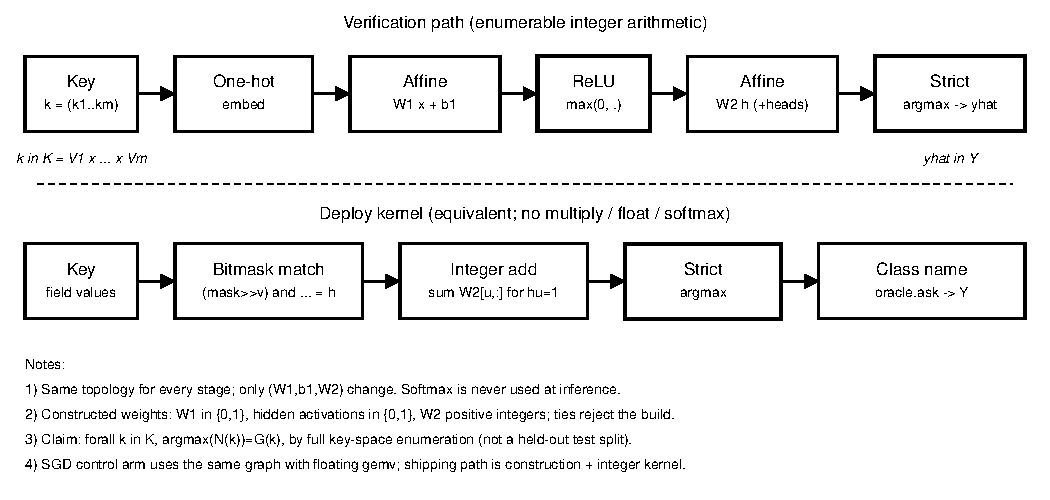
\includegraphics[width=1\textwidth,height=\textheight]{figures/fig1-deterministic-intnet.pdf}
\caption{Deterministic integer feed-forward network: verification path (top) and deployment kernel (bottom). The key space is a finite product \(K\); the output is the class name given by strict argmax.}
\end{figure}

Verification runs every key with integer gemv semantics: one-hot input, integer affine, \(\max(0,\cdot)\), integer affine, strict argmax. The deployment kernel exploits the Boolean \(W_1\) and hidden activations, turning the first layer into a conjunction of stage-local masks and the second into integer addition; it agrees pointwise with the verification path on the domain. It uses no softmax, floating point, multiplication, libm or dynamic memory. The weights of all 18 stages total 9,124 bytes.

\textbf{Axiom of stage-independent representation.} The structure and numeric representation of stage \(s\) are determined by its own finite key domain, vocabularies, output heads and value ranges; other stages impose no common shape. Construction chooses the mask width with \texttt{maskw(st)} separately for each stage. Q-8 chooses, per stage, the smallest representation by byte size that preserves its outputs and checks the corresponding arithmetic ranges. Stages agree only on category and byte-stream interfaces; they need not share a mask width, weight dtype or accumulator width. The basis is that exactness, \(\forall k\in K_s:N_s(k)=G_s(k)\), is decided separately for each \(s\). Enumeration of one stage neither requires another to use the same structure nor proves that either truth table agrees with C99.

Byte-level reproducibility rests on two facts: \textbf{construction is deterministic} --- the same truth tables yield byte-identical weights; and \textbf{inference is integer-only} --- within the kernel's integer width and accumulation range, the result for a given input is unique. Together they make cross-target folding (§6.2) and the self-hosting fixed point (§5.3) possible; consistency across machines and compilers must still be verified on the target platforms.

\subsection{Formal obligations}\label{formal-obligations}

\begingroup\small\setlength{\tabcolsep}{4pt}

\stepcounter{paperTableAnchor}
\begin{longtable}[]{@{}
  >{\raggedright\arraybackslash}p{(\columnwidth - 4\tabcolsep) * \real{0.1153}}
  >{\raggedright\arraybackslash}p{(\columnwidth - 4\tabcolsep) * \real{0.4122}}
  >{\raggedright\arraybackslash}p{(\columnwidth - 4\tabcolsep) * \real{0.4726}}@{}}
\toprule\noalign{}
\begin{minipage}[b]{\linewidth}\raggedright
Proposition
\end{minipage} & \begin{minipage}[b]{\linewidth}\raggedright
Content
\end{minipage} & \begin{minipage}[b]{\linewidth}\raggedright
Discharged by
\end{minipage} \\
\midrule\noalign{}
\endhead
\bottomrule\noalign{}
\endlastfoot
\textbf{P-8} & Every total function \(G:K\to Y\) has an exact network & Lean \texttt{naive\_exact} (restates a known result) \\
\textbf{P-3} & Released network ≡ truth table & Full-domain enumeration of the released integer network; \texttt{decision\_list\_exact} proves only the globally monochrome first-hit subcase \\
\textbf{P-1} & Query discipline (Definition 3) & Engineering discipline; premise of P-5 \\
\textbf{P-5} & Network-driven ≡ table-driven & Lean \texttt{cong\_of\_pointwise}, \texttt{p5\_of\_p3\_trace} (under P-1 and P-3) \\
\textbf{P-2} & Every queried key ∈ \(K_s\) & Runtime assertion; a Lean template on a toy walker; open for the full walkers \\
\textbf{P-6} & Truth table ≡ C99 semantics & External referees (§6.3); not claimed \\
\textbf{P-7} & Observable behaviour on six targets equals the reference VM & Empirical folding, fault injection and native suites \\
\end{longtable}

\addtocounter{table}{-1}

\endgroup

Deliberately out of scope: machine proofs of the self-hosting fixed point and the six ABIs, a proof that the truth tables equal C99, and complexity arguments for the minimum number of units.

\section{From Decisions to a Pipeline: the Network Compiler}\label{from-decisions-to-a-pipeline-the-network-compiler}

\subsection{Partitioning principle: shape, not difficulty}\label{partitioning-principle-shape-not-difficulty}

A decision that is a function from finite keys to finite classes goes into a table. Work that depends on unbounded structure (nesting, recursion, address arithmetic) goes to finite control and generic storage, but only the declared finite transition choices are represented by the constructed network. In the decision-network instance, the deployed C code reads the enumerated DENSE answer table rather than evaluating weights for each query. A common division is \textbf{structure proposes, the table decides}: in peephole optimisation, structural code finds a candidate instruction pair and computes their relation (same slot, constant operand, jump to next, dead destination register); whether to rewrite, and how, is answered by the table. Operator precedence, operation classes, and the mapping from operator and signedness to instruction variant were all hard-coded at first and later moved into tables.

\subsection{Pipeline structure}\label{pipeline-structure}

The network compiler splits compilation into seven \textbf{byte-stream-in, byte-stream-out} stages. Each is a finite transition function constructed from declared rules, compiled into an integer threshold network, and run by the same generic executor:

\begingroup\small\setlength{\tabcolsep}{4pt}

\stepcounter{paperTableAnchor}
\begin{longtable}[]{@{}
  >{\raggedright\arraybackslash}p{(\columnwidth - 4\tabcolsep) * \real{0.1495}}
  >{\raggedright\arraybackslash}p{(\columnwidth - 4\tabcolsep) * \real{0.4073}}
  >{\raggedright\arraybackslash}p{(\columnwidth - 4\tabcolsep) * \real{0.4432}}@{}}
\toprule\noalign{}
\begin{minipage}[b]{\linewidth}\raggedright
Stage
\end{minipage} & \begin{minipage}[b]{\linewidth}\raggedright
Input → output
\end{minipage} & \begin{minipage}[b]{\linewidth}\raggedright
Main responsibilities
\end{minipage} \\
\midrule\noalign{}
\endhead
\bottomrule\noalign{}
\endlastfoot
Preprocessing & source bytes → preprocessed text & line splicing and comments, directives, macro expansion and rescanning, conditional expressions, inclusion \\
Lexing & preprocessed text → typed token stream & keywords and type words, identifiers and operators, literals, longest match \\
Parsing & token stream → tape & declarations and scope, types and conversions, precedence, statements and control, initialisation, calls \\
Optimisation & tape → tape & stack operations to register moves, basic blocks and liveness, peephole fusion \\
Pruning & tape → tape & conservatively removes unreachable whole functions on the image and execution routes, keeping data; public tape output bypasses this stage \\
Lowering & tape → target instructions and data & ABI, register mapping, system-call gates, data layout and relocation \\
Encoding and image & target instructions → ELF / Mach-O / PE (or an in-memory image) & instruction encoding, branch layout, relocation, headers and segments, Mach-O signing \\
\end{longtable}

\addtocounter{table}{-1}

\endgroup

The tape is a target-independent intermediate representation: eight 64-bit registers (one is the stack pointer) and 71 operations in the current \texttt{SHAPE} manifest. Floating-point values travel as IEEE bit patterns in general registers. Tape operation encodings do not bind an ISA; lowering and host-interaction boundaries still handle target ABI facts.

\textbf{One executor step.} The current control state selects an observation bank; the observation is the next input byte, the top of the continuation stack, or the comparison result of the previous action; the network maps the observation to the next state and an action-sequence index; the executor then performs the generic actions of that sequence: advance, mark and rewind, register and indexed-memory reads and writes, output, push and pop, string interning. The executor contains no primitive specific to C, the tape, an instruction set or an image format.

\textbf{Network form.} These networks use an ordered-threshold representation per state: the units of an observation bank are sorted by threshold, and the next state and action index are a base value plus the accumulated differences of the activated units. It is the same method as the cube networks of §3, in a different form: the former suits finite control over byte streams, the latter classification over multi-field discrete descriptions.

\subsection{Two runtime improvements that change no answer}\label{two-runtime-improvements-that-change-no-answer}

Profiling showed that a program containing only \texttt{\#include\ \textless{}stdio.h\textgreater{}} took 3.29M steps in the parsing stage and scanned 602 million threshold units, 97\% of them in a single state --- continuation return.

\textbf{Threshold-prefix evaluation.} Thresholds within a bank are strictly increasing (the loader rejects anything else), so the units activated by an observation always form a prefix. The executor binary-searches the prefix length and accumulates only those differences --- the same network and the same sum, with no answer table stored.

\textbf{Declared returns.} Rows of a stack-keyed bank of the form ``continuation k → k, sharing one action sequence'' mean ``pop and continue at the state the stack names''. The continuation alphabet of a fixed stage is finite; unbounded stack height does not make the top observation an infinite decision. The constructor factors these rows into a declared return set and a generic pop action, building threshold units only for the remaining rows. The return fast path and threshold path together constitute the complete controller. The finite-domain factoring argument in §2.2 applies to both paths; weights alone do not describe this controller. The network--table check still compares every observation, returns included (1,549,292 in the parsing stage), and is fully equal before and after the change.

With both changes, compiling \texttt{fib.c} and the compiler's own source dropped from 10.2× and 25.0× the classic route to 3.9× and 12.8× (§7.2).

\subsection{What is not the model}\label{what-is-not-the-model}

Command-line handling, file and resource adaptation, package reading and checking, and network decompression and loading are classic code. In the decision-network instance, \texttt{src/front\_parse.c::inf} reads DENSE, a table generated by enumerating the constructed networks; direct inference is checked against it, not used for each runtime query. Accordingly, calling this work a neural-network-based compiler is anchored on constructor weights from the TSV table DSL and on T1 (the network equals the table on the declared domain), not on the claim that every product ask in the decision-network instance evaluates live network weights; the DENSE lookup above is a deployment form of that same constructed exact network on the enumerated table---it does not withdraw the naming claim and does not weaken T1. Each threshold bank in a byte-stream stage computes a one-dimensional step function, equivalent to a run-length lookup over that bank's finite key range. In the network-compiler instance, the seven stage transitions do run through constructed networks, but the generic executor also implements storage, action dispatch and declared continuation returns. Selected product routes additionally retain hand-written tape linking (\texttt{src/tapelink.c}), assembly-text handling (\texttt{src/asmtext.c}) and host-forwarding stubs (\texttt{src/fwdstub.c}). The last step of \texttt{-run} is not step-by-step network interpretation either: the host reserves an address chosen by the operating system and hands it to the loaded encoding stage; constructed networks and the generic executor emit the final bound memory image in one pass; the host checks the lengths recorded in it, commits, sets permissions, flushes the instruction cache and jumps to the entry, without interpreting C, the tape or instructions, and without a large language model generating source. The offline constructor still binds target facts, vocabularies and parameterised templates. The constructed networks carry the declared finite stage transitions, not all program code or rule information; ``the runtime path became networks'' and ``the language logic to maintain shrank'' are two conclusions that must be checked separately.

\section{Implementation}\label{implementation}

\subsection{Two instances}\label{two-instances}

\begingroup\small\setlength{\tabcolsep}{4pt}

\stepcounter{paperTableAnchor}
\begin{longtable}[]{@{}
  >{\raggedright\arraybackslash}p{(\columnwidth - 4\tabcolsep) * \real{0.1179}}
  >{\raggedright\arraybackslash}p{(\columnwidth - 4\tabcolsep) * \real{0.4834}}
  >{\raggedright\arraybackslash}p{(\columnwidth - 4\tabcolsep) * \real{0.3986}}@{}}
\toprule\noalign{}
\begin{minipage}[b]{\linewidth}\raggedright
\end{minipage} & \begin{minipage}[b]{\linewidth}\raggedright
Decision-network instance
\end{minipage} & \begin{minipage}[b]{\linewidth}\raggedright
Network-compiler instance
\end{minipage} \\
\midrule\noalign{}
\endhead
\bottomrule\noalign{}
\endlastfoot
Networks & 18 fact tables, cube networks & 33 distinct threshold networks \\
Driver & classic recursive descent, lowering and image writers query networks at decision points & generic executor runs each stage network step by step \\
Size & 8,509 keys, 517 hidden units, 9,124 B of weights (op-74 identity of Table~1; CN draft Table~1 is op-87: 8,769/569) & 129,944 threshold units, 783,938 B compressed (v0.0.9) \\
Fallback & none (query discipline) & none: rejection on out-of-domain keys is an error \\
Distribution & a single C source file & a single 1,233,236 B multi-platform executable (v0.0.9) \\
\end{longtable}

\addtocounter{table}{-1}

\endgroup

\subsection{Size and sharing in the network compiler}\label{size-and-sharing-in-the-network-compiler}

\begingroup\scriptsize\setlength{\tabcolsep}{4pt}

\stepcounter{paperTableAnchor}
\begin{longtable}[]{@{}
  >{\raggedright\arraybackslash}p{(\columnwidth - 16\tabcolsep) * \real{0.1661}}
  >{\raggedleft\arraybackslash}p{(\columnwidth - 16\tabcolsep) * \real{0.0780}}
  >{\raggedleft\arraybackslash}p{(\columnwidth - 16\tabcolsep) * \real{0.1038}}
  >{\raggedleft\arraybackslash}p{(\columnwidth - 16\tabcolsep) * \real{0.0954}}
  >{\raggedleft\arraybackslash}p{(\columnwidth - 16\tabcolsep) * \real{0.0868}}
  >{\raggedleft\arraybackslash}p{(\columnwidth - 16\tabcolsep) * \real{0.1038}}
  >{\raggedleft\arraybackslash}p{(\columnwidth - 16\tabcolsep) * \real{0.0954}}
  >{\raggedleft\arraybackslash}p{(\columnwidth - 16\tabcolsep) * \real{0.1587}}
  >{\raggedleft\arraybackslash}p{(\columnwidth - 16\tabcolsep) * \real{0.1120}}@{}}
\caption{Per-stage structure of the network compiler (v0.0.9, \texttt{osx/arm64} -O2 image route, static). The package has 33 distinct networks and 1,082 stage-route rows; figures from the \href{https://github.com/partnernetsoftware/unisacc/blob/3b971eaa14321d27faf0346b25d5c00d358b3b98/archive/research/r9/r9-pipeline-structure-prune.json}{structure audit}.}\tabularnewline
\toprule\noalign{}
\begin{minipage}[b]{\linewidth}\raggedright
Stage
\end{minipage} & \begin{minipage}[b]{\linewidth}\raggedleft
States
\end{minipage} & \begin{minipage}[b]{\linewidth}\raggedleft
Sequences
\end{minipage} & \begin{minipage}[b]{\linewidth}\raggedleft
Expanded actions
\end{minipage} & \begin{minipage}[b]{\linewidth}\raggedleft
Stored actions
\end{minipage} & \begin{minipage}[b]{\linewidth}\raggedleft
Threshold units
\end{minipage} & \begin{minipage}[b]{\linewidth}\raggedleft
Return banks / keys
\end{minipage} & \begin{minipage}[b]{\linewidth}\raggedleft
Raw / compressed B
\end{minipage} & \begin{minipage}[b]{\linewidth}\raggedleft
Package references
\end{minipage} \\
\midrule\noalign{}
\endfirsthead
\toprule\noalign{}
\begin{minipage}[b]{\linewidth}\raggedright
Stage
\end{minipage} & \begin{minipage}[b]{\linewidth}\raggedleft
States
\end{minipage} & \begin{minipage}[b]{\linewidth}\raggedleft
Sequences
\end{minipage} & \begin{minipage}[b]{\linewidth}\raggedleft
Expanded actions
\end{minipage} & \begin{minipage}[b]{\linewidth}\raggedleft
Stored actions
\end{minipage} & \begin{minipage}[b]{\linewidth}\raggedleft
Threshold units
\end{minipage} & \begin{minipage}[b]{\linewidth}\raggedleft
Return banks / keys
\end{minipage} & \begin{minipage}[b]{\linewidth}\raggedleft
Raw / compressed B
\end{minipage} & \begin{minipage}[b]{\linewidth}\raggedleft
Package references
\end{minipage} \\
\midrule\noalign{}
\endhead
\bottomrule\noalign{}
\endlastfoot
Preprocessing & 1,836 & 1,396 & 10,641 & 6,159 & 3,400 & 1 / 231 & 62,762 / 24,235 & 20 \\
Lexing & 403 & 8,179 & 17,256 & 16,533 & 11,259 & 0 / 0 & 131,908 / 23,064 & 120 \\
Parsing & 6,440 & 17,350 & 71,714 & 55,774 & 23,044 & 1 / 1,562 & 462,815 / 110,632 & 108 \\
Optimisation & 904 & 403 & 6,912 & 6,784 & 1,053 & 1 / 65 & 45,128 / 12,621 & 72 \\
Pruning & 322 & 166 & 1,739 & 1,707 & 297 & 1 / 13 & 11,251 / 4,132 & 144 \\
Lowering & 1,572 & 809 & 15,095 & 5,537 & 937 & 1 / 447 & 39,840 / 13,454 & 24 \\
Encoding and image & 1,937 & 840 & 9,234 & 7,888 & 1,517 & 1 / 333 & 62,960 / 19,694 & 13 \\
\end{longtable}

\endgroup

``Expanded actions'' is the sum of actions over all static sequences after expanding shared prefixes; ``stored actions'' counts only each record's own action suffix; neither is an execution count. The seven stages total 13,414 states, 29,143 sequences, 132,591 expanded actions, 100,382 stored actions, 41,507 threshold units and 6 return banks / 2,651 keys; 816,664 B raw, 207,832 B compressed. Counting each of the 33 networks once, the package has 56,701 states, 81,777 sequences, 456,158 expanded actions, 307,529 stored actions, 129,944 threshold units and 31 return banks / 10,774 keys; 2,620,844 B raw, 783,938 B compressed. Compressed sizes exclude the package directory and record headers; shared networks are not counted once per reference.

The lexing, parsing, optimisation, pruning and multi-file framing networks are shared by all six targets; each target owns two preprocessing variants, one lowering network and one encoding network. The same preprocessing variant differs across targets only in predefined macros (record-level Jaccard 0.998--0.999, measured on the pre-pruning candidate), which suggests further room for sharding (§8). ``Shared'' here means construction flow and routing for some stages, \textbf{not} one invariant weight blob across OS and architecture: tables bind target facts and encodings before release, with per-target lowering and encoding variants. We do not claim an unproved ``single network'' cross-platform invariant.

v0.0.9 passed 193/193 local gates on the final frozen source, with a six-target × three-program smoke test and execution evidence after macOS signing and packaging; which platforms ran natively or under emulation, and that Windows self-hosting was not verified, are recorded in the \href{https://github.com/partnernetsoftware/unisacc/blob/3b971eaa14321d27faf0346b25d5c00d358b3b98/archive/research/r9/r9-release-acceptance.json}{release receipt}.

\subsection{Self-hosting}\label{self-hosting}

The decision-network instance self-hosts in three layers, each judged by byte equality:

\begin{enumerate}
\def\labelenumi{\arabic{enumi}.}
\tightlist
\item
  \textbf{Front-end fixed point.} The compiler compiles itself to tape: A compiles itself to B, B compiles itself to C; we require B = C, identical to the result of an independent implementation (the Python front end).
\item
  \textbf{Back-end closure.} For every probe and target, the image written by the C back end must be byte-identical to the image written by the Python back end from the same tape: 94 probes × 6 targets, 564/564; the compiler itself 6/6.
\item
  \textbf{Native self-hosting without Python.} The native compiler writes itself as N1, N1 writes N2, N2 writes N3; we require N1 = N2 = N3 and consistent cross output for the other five targets. This holds on osx/arm64, lnx/arm64, lnx/x86-64, win/arm64 and win/x86-64 (the latter under system emulation), without invoking Python.
\end{enumerate}

Byte-identical bootstrap (N1 = N2 = N3) asserts only unsigned successive-generation binary identity under the named checks; it is not a semantic self-hosting theorem, not C99 completeness, and not a proof that tables agree with C semantics (table semantics still rest on external referees and the stated boundaries).

The network compiler self-hosts its driver with a fixed network package (N1 = N2 = N3 on macOS arm64); this does not include self-construction of the network package or of the multi-platform container.

\subsection{R10 development evidence (not a replacement release baseline)}\label{r10-development-evidence-not-a-replacement-release-baseline}

Table 2 and the performance tables retain the v0.0.9 release baseline. An R10 development candidate adds a \texttt{nativeabi} carrier-certification stage: the network maps an original type graph and target facts to a carrier certificate; the host executes the declared data moves and calls. The natural 16-byte union domain preserves logical parameter count, object extent and alignment 4/8, distinguishing integer/SSE lanes and ARM HFAs by target. The model has 1,332 states, with network=table over all 343,400 observations and 310 independent graph-oracle cases. Across two macOS ISAs, nine layouts, four register-pressure patterns and both call directions, 144 actual variants passed ASan/UBSan and 100 repetitions at each of three optimisation levels: 43,200 native calls and 21,600 SCRIPT callbacks. A mixed-register boundary failure with system macOS x86\_64 libffi is retained separately; the actual calls pass with the pinned official 3.5.2 dependency. Network--table equality does not prove this host ABI fact. The development artifact is 1,116,367 B; all 24 deployed networks pass full-domain checks and 28 affected gates pass (\href{https://github.com/partnernetsoftware/unisacc/blob/3b971eaa14321d27faf0346b25d5c00d358b3b98/archive/research/r10/r10-union16-candidate-evidence.json}{candidate}, \href{https://github.com/partnernetsoftware/unisacc/blob/3b971eaa14321d27faf0346b25d5c00d358b3b98/archive/research/r10/r10-union16-qualified-public-evidence.json}{public calls}, \href{https://github.com/partnernetsoftware/unisacc/blob/3b971eaa14321d27faf0346b25d5c00d358b3b98/archive/research/r10/r10-ffi-provider-delivery-evidence.json}{dependency counterexample and delivery}). This is not a v0.0.10 release claim or qualification of arbitrary union/BANK, bitfields, wide FP or all six platform ABIs; those remain development obligations.

\subsection{Subsequent evidence and open obligations in v0.0.13--v0.0.14}\label{subsequent-evidence-and-open-obligations-in-v0.0.13v0.0.14}

This is an incremental release record. Tables 2 and 4 retain v0.0.9 as an identity-fixed historical baseline; network counts, bytes and timings from different versions are not combined into one measurement. The unsigned v0.0.13 candidate was 1,190,297 B; each of its 361 local gates passed and the six-target hosted demo matrix passed. The unsigned v0.0.14 candidate was 1,288,064 B. Its publicly signed \texttt{unisacc.com} was 1,303,840 B, SHA-256 \texttt{\seqsplit{c229cebf6cd58ca018fece7f0d3cb142e3a6a52774ac7306f8d5423248b055df}}. Each of 365 local gates passed, and the six-target hosted demo matrix passed. These are finite test results, not a proof of C99 correctness (\href{https://github.com/partnernetsoftware/unisacc/blob/3b971eaa14321d27faf0346b25d5c00d358b3b98/archive/research/r13/r13-release-acceptance.json}{v0.0.13 receipt}, \href{https://github.com/partnernetsoftware/unisacc/blob/3b971eaa14321d27faf0346b25d5c00d358b3b98/research/r14-release-acceptance.json}{v0.0.14 receipt}).

v0.0.14 added \href{https://github.com/partnernetsoftware/unisacc/blob/3b971eaa14321d27faf0346b25d5c00d358b3b98/docs/tapebin-v1.md}{tapebin v1}, a canonical binary representation of target-independent tape operation records. The header also records \texttt{origin\_target}, preserving which target's front-end semantics produced the tape. The 71 opcode shapes are generated from \texttt{unisa/tape.py} and checked by the \texttt{tapebin-shape} gate. \texttt{tapebin-roundtrip} compares structured records and binary bytes through round trips. \texttt{com-tapebin} compares C-reference, Python and product encoders on the same textual tape, and checks that the product both emits and reads its own binary tape. Stability of canonical binary bytes does not mean recovering arbitrary whitespace or comments in hand-written text.

The N22 bootstrap check produced identical \textbf{unsigned} files from the seed, second stage and third stage, each with SHA-256 \texttt{\seqsplit{3d86639072f5d5625baa849041d1919863bf03c8bb4a2e684638ca83ce3f063a}}. The publicly signed \texttt{.com} has different bytes and is not part of that fixed point. The C99 clause ledger, \href{https://github.com/partnernetsoftware/unisacc/blob/3b971eaa14321d27faf0346b25d5c00d358b3b98/tests/c99/clauses.tsv}{\texttt{tests/c99/clauses.tsv}}, records evidence by normative subclause: among 98 language subclauses, 95 are covered, one partial and two unsupported; among 16 environment subclauses, 13 are covered, two partial and one unsupported; among 361 library subclauses, 127 are covered, 43 partial and 191 unsupported. The 59/59 result from \texttt{c99.sh} is a probe result and cannot replace these coverage denominators.

For the \textbf{v0.0.14} release identity, two named R14-8 byte-level obligations remain. For \texttt{b\_compound} and \texttt{b\_pp2}, global compound-literal paths in E3 produce tapes different from the C reference and therefore different images on all six targets; measured program outputs agree with the system compiler. \texttt{exec/c/chain.knownfail} marks either case becoming equal as a revived failure, requiring its ledger line to be removed. We therefore claim byte-level parity only for the listed measured inputs outside these two entries, and retain both as open obligations (\href{https://github.com/partnernetsoftware/unisacc/blob/3b971eaa14321d27faf0346b25d5c00d358b3b98/archive/plans/v0.0.14.md}{R14-8 record}). §5.7 records later tape-level progress on a development candidate; it does not claim six-target image closure.

\subsection{v0.0.18--v0.0.19 increments (released with v0.0.19; not a replacement baseline)}\label{v0.0.18v0.0.19-increments-released-with-v0.0.19-not-a-replacement-baseline}

0.0.18 was not released on its own; its completed items shipped with 0.0.19 on 2026-10-01. The publicly signed \texttt{unisacc.com} is 1,922,560 B, SHA-256 \texttt{ad1d87e9…}; the unsigned candidate \texttt{de39c9bb…} satisfies seed = stage 2 = stage 3. Each of 415 local gates passed once, the release check passed on six runners, and both Windows targets rebuilt themselves byte-identically in local virtual machines (\href{https://github.com/partnernetsoftware/unisacc/blob/3b971eaa14321d27faf0346b25d5c00d358b3b98/research/r19-release-acceptance.json}{v0.0.19 receipt}). The feature figures below are still development-tree measurements; Tables 2 and 4 are not remeasured for v0.0.19 (see §8.1).

\textbf{Assembly text and a bundled assembler.} \texttt{-S\ -b\ lnx/ARCH\ -o\ F.s} disassembles the ELF object written by the back end into GNU assembly, and \texttt{unisacc\ as} reads it back into the same object. Both directions share one encoder: every disassembled instruction is reassembled, and it is printed as a mnemonic only if bytes and relocations are identical; otherwise it falls back to \texttt{.byte}/\texttt{.inst}. Round-trip equality therefore holds by construction, and the gate only counts fallbacks. Before the work began we measured how canonical the back end's encodings are: the objects of 186 probes were disassembled with objdump, reassembled with the system assembler and compared instruction by instruction. On arm64 all of about 1.43 million instructions were byte-identical; on x86-64, of about 1.45 million, only two kinds differed from the assembler's default choice --- a redundant REX 0x40 on narrow stores, and long jumps the assembler would shorten --- and these are written with the \texttt{\{rex\}} and \texttt{\{disp32\}} pseudo-prefixes. The 372 corpus objects across the two targets round-trip byte-identically with 0 fallbacks; the system assembler accepts the text, and \texttt{.text}, relocations and \texttt{.data} match the original object.

\textbf{Moving data out of the tables.} System-call names used to be vocabulary of the \texttt{op} field in four truth tables (abi, enc, combo, isel), so each new call enlarged the key domain of four stages and forced a full rebuild: adding two calls touched 60 files and about 6,500 lines (mostly re-emitted weights and kernel). After 0.0.19 added a generic gate that takes the call number as the first argument, call numbers became constants in the headers, selected by OS and architecture. The dozen or so process functions added afterwards (fork, execvp, waitpid, pipe, dup2, getcwd and others) changed only headers, left the weight bytes unchanged, and agree with cc on osx/arm64, cc under Rosetta on x86-64, and gcc on lnx/arm64. The lesson matches ``Representation versus maintenance cost'' in §8: \textbf{a finite constant mapping is data; putting it into a constructed network adds no trust, only rebuild cost.}

\textbf{Host forwarding in run mode.} Under \texttt{-run} on macOS, an external function that has a prototype, no definition and no bundled body gets a C forwarding stub generated by the front end (dlsym plus the system libffi), compiled again as a final unit; a missing host symbol is reported by name. This exposed a layout precondition: when the bundled \texttt{struct\ tm} lacked two of the host's fields, \texttt{gmtime\_r} wrote past the end and crashed --- forwarding requires bundled struct layouts to match the host. Writing files and cross-target compilation do not forward and still use only the bundled library. The network product takes the same path: under a dedicated resource, stage E3 emits a sidecar of ``undefined reachable calls + type signatures'', and the driver decodes it and generates the same stub text with stub-splicing code shared with the reference; variadic calls, structs by value and calls without prototypes are refused by name rather than having their types guessed. On the development candidate, product, reference and cc agree three ways.

\textbf{Bundled library filled out along Linux interfaces.} In the same period, following a user-measured list, we added the full errno set (values follow the target kernel, one column each for Linux and macOS, so cross-target compilation does not write macOS's EAGAIN=35 into a Linux program), fsync/dup/access/readlink/symlink/rmdir/fdopen, telldir/seekdir, and gmtime/localtime/mktime/strftime (localtime reads TZif time-zone data). All of these changed only headers; each has a probe compared against the native cc (osx/arm64) and gcc (lnx/arm64).

\textbf{Construction time.} Construction of all stages dropped from 30 s to 11 s, with \texttt{built.json} and the shipped weights byte-identical: stages are constructed in parallel, cube keys are memoised, and known literal masks are reused during expansion.

\subsection{v0.0.20 increments (released; not a replacement baseline)}\label{v0.0.20-increments-released-not-a-replacement-baseline}

Released with v0.0.20 on 2026-10-01: the publicly signed \texttt{unisacc.com} is 1,944,384 B, SHA-256 \texttt{3a201488…}; the unsigned candidate \texttt{b275b86e…} satisfies seed = stage 2 = stage 3, and each of 418 local gates passed once (\href{https://github.com/partnernetsoftware/unisacc/blob/3b971eaa14321d27faf0346b25d5c00d358b3b98/research/r20-release-acceptance.json}{v0.0.20 receipt}).

\textbf{Whole-program facts at link time.} Separately compiled unit tapes used not to record whether a global object has an initialiser, so when two units each gave the same object an initialiser, the linker merged them into one object whose final value depended on link order. Now the first record of every \texttt{-funit} unit is \texttt{.unit\ 2}, and each definition with an initialiser carries an extra \texttt{.gdef} record. The linker refuses by name when an object has two initialisers, or when an object is only declared \texttt{extern} and no unit defines it. Old objects without the version record are also refused: they cannot prove that they carry no initialisers, and guessing that they are ``all tentative definitions'' would bring back the silent merge. The one-step whole-program path likewise reports by name an object that is only declared \texttt{extern} but is read.

\textbf{Structured refusals.} Coverage refusals now write one machine-readable line before the human-readable diagnostic: \texttt{UNCOVERED}, stage, key, position, source position, construct and reason --- seven columns, with \texttt{-} for missing fields. The reference side first covers constructs refused by name (the first case is \texttt{\_Complex}, previously misreported as an unknown identifier). The reference implementation does not run the same δ tables, so only decisions that reuse the same gold table require both sides to agree on the key; other gaps are judged by same-source construct probes plus the product's located refusals.

\textbf{The two remaining byte differences (v0.0.20 development candidate).} For the two named differences registered at v0.0.14 (§5.5) we reproduced the first differing byte of each: in \texttt{b\_compound}, the data records of a compound-literal object were placed inside the instruction stream (only 4 lines moved); in \texttt{b\_pp2}, the reference omits a same-type compound literal used as the whole initialiser, while the product first builds the object and then copies it. The two have different root causes and cannot both be fixed by one ordering rule (\href{https://github.com/partnernetsoftware/unisacc/blob/3b971eaa14321d27faf0346b25d5c00d358b3b98/archive/research/r20/r20-3b-first-diffs.md}{first-difference record}). On a \textbf{v0.0.20 development candidate} (not a published release identity), after separate fixes to product E3, the tapes of both cases are byte-identical to the reference, \texttt{exec-chain} is 264/264 equal, and the v0.0.14 known-difference list is cleared at tape level; six-target images still await checking on a candidate build before the v0.0.14 ledger lines close.

\textbf{Bundled library.} Added \texttt{struct\ timespec}, \texttt{clock\_gettime}, \texttt{nanosleep}, \texttt{sleep}/\texttt{usleep} and the \texttt{execl} family, again changing only headers. A new check: each bundled header compiles when included alone (host, lnx/x86\_64, win/x86\_64). Its first run found \texttt{poll} missing from \texttt{sys/select.h} on Windows --- another instance of the ``unit combination'' class of defects.

\subsection{v0.0.21 development increments (unreleased)}\label{v0.0.21-development-increments-unreleased}

The following is development-tree work after v0.0.20 was published (2026-10-01). It is not a release result and has not passed the release gates or a candidate build.

\textbf{libc direction (owner, 2026-10-02).} The home-grown libc no longer grows: the bundled library is to become an external libc package rather than live inside \texttt{unisacc.com}, and ``add a body when a program needs it'' stops. Functions the system already has are forwarded to the system libc; the \href{https://github.com/partnernetsoftware/unisacc/blob/3b971eaa14321d27faf0346b25d5c00d358b3b98/research/libc-route-table.md}{route table} (design) assigns each family to forward, keep or refuse.

\textbf{Generic forwarding.} The forwarding stubs that were limited to macOS \texttt{-run} are generalised: every function with a prototype, no definition and no bundled body gets a compiler-generated stub (dlsym plus a host call), in written images and under \texttt{-run}, on macOS and Linux (commit \texttt{f0b31b9}). Linux images that forward are written as a minimal dynamic ELF: PT\_INTERP, DT\_NEEDED \texttt{libc.so.6}, and four dl* GLOB\_DAT slots in the same place as the Mach-O eager bind; programs that do not forward keep identical bytes. Development-tree measurements: gethostname, sysconf and getpagesize forwarded correctly on lnx/arm64, lnx/x86\_64, osx/arm64 and osx/x86\_64; the forward suite passes 10/10, including written osx images and lnx/arm64 dynamic ELF images compared against cc/gcc. A cosmopolitan-style POSIX layer for Windows is planned only (\href{https://github.com/partnernetsoftware/unisacc/blob/3b971eaa14321d27faf0346b25d5c00d358b3b98/research/win-posix-plan.md}{design}); it is not implemented.

\textbf{A lesson from the header-standalone check.} The check that each bundled header compiles when included alone ran with library trimming on, so bodies no program used were never compiled and the check missed them. Recompiling every body found \texttt{time.h} calling a helper defined only in \texttt{unistd.h}, and two headers that cannot work on Windows (\texttt{dirent.h}, \texttt{unisacc\_ffi.h}, now refused by name). This is the theme of §7.4: a check covers only what it actually exercises.

\textbf{Real programs keep finding defects.} Making Lua 5.4's single-file build (onelua.c) pass required fixing more than ten defects in the reference front end, each with a probe compared against cc: typedef'd arrays not treated as arrays at declarations; a \texttt{T\ **} struct member indexed in sizeof(T) steps; a call through a function-pointer member dereferenced once too often; member declaration specifiers leaking out of a struct body; an incomplete extern array sized wrongly when defined later (its initialiser cleared the adjacent character-class table); \texttt{\#include} silently dropped after 200 inclusions; a live \texttt{\#error} ignored. setjmp/longjmp became compiler intrinsics (they cannot be forwarded: they must capture the generated code's own frame). None of these constructs is a key of any single table, consistent with §7.4: combinations and real programs are the main source of failures outside the unit of verification. The corpus ratchet therefore passes one more program than 0.0.20.

\textbf{cc interoperation.} Objects written by \texttt{-c} can now call and be called by functions compiled by the system cc: outbound with integer, pointer, floating-point and stack arguments, inbound with integers and pointers (osx/arm64, lnx/arm64, lnx/x86\_64); other signatures are refused by name.

\section{Verification Methodology}\label{verification-methodology}

\subsection{Full-domain enumeration (T1)}\label{full-domain-enumeration-t1}

Every cube network is run with deployment arithmetic on \textbf{every} key of the original domain; any wrong key or tie fails construction and blocks release. On the normal path, the C side of the decision-network instance queries a dense table obtained by enumeration, and an explicit acceptance command compares, one by one, the table answer and the direct inference result for all 20,190 key--head questions (zero differences). Each of the 33 transition networks in the v0.0.9 baseline is checked over its declared observation domain, comparing successor states, action sequences and strings; later releases require their own network count.

\subsection{Byte-level differential testing and six-target folding}\label{byte-level-differential-testing-and-six-target-folding}

After the tape is lowered to six targets, each image is executed by a machine model \textbf{interpreting that target's ABI}: the model holds the architecture's named registers, and the system-call dispatcher recognises only the (OS, call number) produced by lowering, never looking back at the tape. The six (stdout, exit) pairs must agree with each other and with a tape reference VM. To show that 6/6 is not vacuous we inject a fault: removing the class bits of macOS system-call numbers must degrade the result to 4/6. The v0.0.19 \href{https://github.com/partnernetsoftware/unisacc/blob/3b971eaa14321d27faf0346b25d5c00d358b3b98/research/r19-release-acceptance.json}{release receipt} records six hosted runners for the demo matrix, ABI machine-model folding for six targets, and byte-identical Windows self-rebuilds in local virtual machines; it does not publish a per-target matrix of host, Linux VM and Windows VM native runs (§8.1 item 3).

\textbf{Are the networks really deciding?} Tests that compare only answers cannot detect ``a hand-written rule that happens to agree with the table''. Both front ends therefore report how often each stage is queried, and every stage one front end queries on a probe must also be queried by the other. This check caught a drift in which one front end queried only three stages.

\subsection{External referees}\label{external-referees}

Enumeration closes only ``network = table''; it says nothing about ``table = C''. We register a referee for each stage: eight stages have named external referees (preprocessing, parsing, type, ABI, precedence, type info, binary-operator selection, printf conversion), six have only cross-implementation agreement, two have no direct referee yet (scope, irsel --- unnamed in the ledger), and two are not on the main compilation path; the ledger is \texttt{research/referee.tsv}.

\begingroup\small\setlength{\tabcolsep}{4pt}

\stepcounter{paperTableAnchor}
\begin{longtable}[]{@{}
  >{\raggedright\arraybackslash}p{(\columnwidth - 2\tabcolsep) * \real{0.3050}}
  >{\raggedright\arraybackslash}p{(\columnwidth - 2\tabcolsep) * \real{0.6950}}@{}}
\toprule\noalign{}
\begin{minipage}[b]{\linewidth}\raggedright
External referee
\end{minipage} & \begin{minipage}[b]{\linewidth}\raggedright
Coverage and limits
\end{minipage} \\
\midrule\noalign{}
\endhead
\bottomrule\noalign{}
\endlastfoot
Preprocessing & Macro-expansion tokens aligned one by one with the host \texttt{cc\ -E\ -P} (\texttt{exec/pp/macrocheck.py}, \texttt{tests/ccparity.sh}) \\
Parsing & The (line, kind) diagnostic set equals the host \texttt{cc\ -Wall} in both directions (\texttt{tests/warn.sh}, probes and corpus) \\
Type & Result types checked with the host cc's C11 \texttt{\_Generic}; 1,400 of 4,275 keys \\
ABI & Numbers checked against host system-call headers; only the actual host OS and architecture \\
Precedence & 324 ordered operator pairs: 291 distinguishable on the chosen constants and consistent, 33 indistinguishable \\
Type info & Sizes of 11 types; signedness and narrowness of 8 integer types \\
Binary-operator selection & The host cc compares signed and unsigned 64-bit results per operator: 7 of 16 operators depend on signedness, and the table names an unsigned flavour exactly there (\texttt{tests/binsel\_audit.py}) \\
printf conversion & The host printf output shape for the 9 conversion letters matches the routine class the table assigns (\texttt{tests/pfconv\_audit.py}) \\
\end{longtable}

\addtocounter{table}{-1}

\endgroup

The accurate statement is therefore: 18/18 stages have an enumeration proof of network = table, and 8/18 stages have external referees of stated coverage. \textbf{Measurement} is a third kind of evidence: the peephole cost table is revised from measurements (§7.4), but that stage is registered in the ledger as cross-implementation agreement and is not counted among the six.

\section{Evaluation}\label{evaluation}

We answer four questions. \textbf{RQ1}: Can the method support a real compiler? \textbf{RQ2}: What does it cost? \textbf{RQ3}: How does construction compare with training? \textbf{RQ4}: Does this verification discipline find defects that conventional testing misses?

\subsection{RQ1: Correctness and coverage}\label{rq1-correctness-and-coverage}

\begingroup\small\setlength{\tabcolsep}{4pt}

\stepcounter{paperTableAnchor}
\begin{longtable}[]{@{}
  >{\raggedright\arraybackslash}p{(\columnwidth - 4\tabcolsep) * \real{0.2285}}
  >{\raggedright\arraybackslash}p{(\columnwidth - 4\tabcolsep) * \real{0.3560}}
  >{\raggedright\arraybackslash}p{(\columnwidth - 4\tabcolsep) * \real{0.4154}}@{}}
\caption{Acceptance record of the decision-network instance}\tabularnewline
\toprule\noalign{}
\begin{minipage}[b]{\linewidth}\raggedright
Item
\end{minipage} & \begin{minipage}[b]{\linewidth}\raggedright
Criterion
\end{minipage} & \begin{minipage}[b]{\linewidth}\raggedright
Result
\end{minipage} \\
\midrule\noalign{}
\endfirsthead
\toprule\noalign{}
\begin{minipage}[b]{\linewidth}\raggedright
Item
\end{minipage} & \begin{minipage}[b]{\linewidth}\raggedright
Criterion
\end{minipage} & \begin{minipage}[b]{\linewidth}\raggedright
Result
\end{minipage} \\
\midrule\noalign{}
\endhead
\bottomrule\noalign{}
\endlastfoot
Stage accuracy & Full-domain enumeration & all 18 stages 1.000 \\
Truth table vs cc & Type table key by key against the system cc & 1,400 keys: 1,399 agree, 1 intentional deviation \\
External corpus c-testsuite & Output equals the system cc & 216 of 220 pass, 0 errors; 4 outside the supported subset \\
C99 probes & One by one against the system cc & 59/59 \\
Differential tests & Against the system cc & 93/93 \\
Optimisation levels & -O0/-O1/-O2 output equals cc -O2 & 279/279 \\
Two optimisers agree & Same tape through both optimisers & 190/190 \\
Real library code & Known-answer tests of crypto-algorithms etc. & 11/11 \\
Back-end closure & Images byte-identical to the reference back end & 564/564; the compiler itself 6/6 \\
Float formatting & \texttt{\%f/\%e/\%g} bit-identical to the platform libc & identical; no floating-point arithmetic in the formatter \\
\end{longtable}

\endgroup

Network compiler v0.0.9: all 33 deployed networks are equal to their tables over their whole domains; 193/193 local gates pass (including byte-level comparison with the classic reference on the gate corpus); a six-target × three-program smoke test passes, with some targets executed under emulation (scope in the \href{https://github.com/partnernetsoftware/unisacc/blob/3b971eaa14321d27faf0346b25d5c00d358b3b98/archive/research/r9/r9-release-acceptance.json}{release receipt}).

\subsection{RQ2: Cost}\label{rq2-cost}

\textbf{Size.} The single-file product shrank from 5,388,402 B (v0.0.8) to 1,233,236 B (v0.0.9, −77.1\%). The reduction comes from three changes that alter no network answer: networks are stored as binary records, compressed and checksummed one by one; action sequences reference shared prefixes; and \texttt{-run} emits the final bound memory image in one pass. After each change the full-domain network--table check was repeated.

\textbf{Speed.} Table 4 reports medians of five fresh processes on the same machine (the compiler-source row is a single run). The four rows are \textbf{not} one same-identity benchmark: rows 1--2 used pre-pruning candidate \texttt{c4993fd0…}, rows 3--4 used product \texttt{c94cf5fe…} after two runtime improvements (Appendix A). Summarising the ratio column as roughly 4--17$\times$ is only a historical cross-artifact band. On v0.0.9, compiling and running \texttt{calc.c} takes 0.177 s and starting a minimal program 0.029 s, level with the first two rows: pruning gave no measurable speed-up on this input (\href{https://github.com/partnernetsoftware/unisacc/blob/3b971eaa14321d27faf0346b25d5c00d358b3b98/archive/research/r9/r9-prune-product-bench.json}{receipt}).

\begingroup\small\setlength{\tabcolsep}{4pt}

\stepcounter{paperTableAnchor}
\begin{longtable}[]{@{}
  >{\raggedright\arraybackslash}p{(\columnwidth - 6\tabcolsep) * \real{0.5348}}
  >{\raggedleft\arraybackslash}p{(\columnwidth - 6\tabcolsep) * \real{0.1800}}
  >{\raggedleft\arraybackslash}p{(\columnwidth - 6\tabcolsep) * \real{0.1655}}
  >{\raggedleft\arraybackslash}p{(\columnwidth - 6\tabcolsep) * \real{0.1196}}@{}}
\caption{Network-compiler timing relative to the classic reference (historical; rows 1--2: \texttt{c4993fd0…}; rows 3--4: \texttt{c94cf5fe…})}\tabularnewline
\toprule\noalign{}
\begin{minipage}[b]{\linewidth}\raggedright
Workload
\end{minipage} & \begin{minipage}[b]{\linewidth}\raggedleft
Classic reference
\end{minipage} & \begin{minipage}[b]{\linewidth}\raggedleft
Network compiler
\end{minipage} & \begin{minipage}[b]{\linewidth}\raggedleft
Ratio
\end{minipage} \\
\midrule\noalign{}
\endfirsthead
\toprule\noalign{}
\begin{minipage}[b]{\linewidth}\raggedright
Workload
\end{minipage} & \begin{minipage}[b]{\linewidth}\raggedleft
Classic reference
\end{minipage} & \begin{minipage}[b]{\linewidth}\raggedleft
Network compiler
\end{minipage} & \begin{minipage}[b]{\linewidth}\raggedleft
Ratio
\end{minipage} \\
\midrule\noalign{}
\endhead
\bottomrule\noalign{}
\endlastfoot
\texttt{calc.c}: compile and run in memory & 0.0108 s & 0.179 s & 16.6× \\
Minimal program: start-up & 0.0032 s & 0.029 s & 9.2× \\
\texttt{fib.c}: compile to image & 0.0797 s & 0.312 s & 3.9× \\
Compiler's own source: compile to image & 0.790 s & 10.15 s & 12.8× \\
\end{longtable}

\endgroup

This is the real price of interpreting finite control step by step with a generic executor, and we do not hide it. The main source has been located: the 2.7 KB source of \texttt{calc.c} expands to about 67 KB after automatic header inclusion, about 96\% of which is the bundled C library, processed by every later stage. We therefore added a switch that keeps only the library functions a program needs: every library function body in the headers is guarded, and the preprocessing stage defines the guards for the closure, over a dependency table derived from the headers, of the names the program actually uses. On the classic reference it shrinks the tape of \texttt{calc.c} from 268 KB to 132 KB and the image from 99 KB to 66 KB; the preprocessing-network implementation is byte-identical to the classic reference on 156 files × both switch states, 312/312.

\textbf{Comparison with conventional compilers (decision-network instance only).} Table 5 is one historical measurement of the \textbf{decision-network instance} on osx/arm64 (minimum of three): classic compilation code consults the enumerated \textbf{DENSE} answer table, not the seven-stage generic executor of the network-compiler pipeline (Table 4). It is \textbf{not} a network-compiler pipeline timing. Every compiler performs the same task --- compiling unisacc itself at -O2 --- and outputs are checked byte for byte.

\begingroup\footnotesize\setlength{\tabcolsep}{4pt}

\stepcounter{paperTableAnchor}
\begin{longtable}[]{@{}lllll@{}}
\caption{Decision-network instance (DENSE lookup) versus tcc and cc --- single workload, not pipeline timing}\tabularnewline
\toprule\noalign{}
unisacc built by & Build time & Resulting binary & That binary compiles unisacc.c & Relative to cc -O2 \\
\midrule\noalign{}
\endfirsthead
\toprule\noalign{}
unisacc built by & Build time & Resulting binary & That binary compiles unisacc.c & Relative to cc -O2 \\
\midrule\noalign{}
\endhead
\bottomrule\noalign{}
\endlastfoot
cc -O2 & 1.81 s & 569,384 B & 0.15 s & 1.0× \\
cc -O0 & 0.15 s & 490,840 B & 0.49 s & 3.3× \\
tcc & 0.02 s & 683,008 B & 0.55 s & 3.7× \\
unisacc -O2 (itself) & 0.15 s & 677,154 B & 0.81 s & 5.4× \\
unisacc -O0 (itself) & 0.10 s & 1,056,930 B & 2.05 s & 13.8× \\
\end{longtable}

\endgroup

On this workload the self-built compiler takes about 1.5× the time of the tcc-built one. The figures are retained for reproducibility (Appendix A); they characterize only the DENSE-backed decision-network instance on one workload, not network-compiler execution (Table 4), and are not submission-grade without remeasurement (§8.1).

\subsection{RQ3: Construction versus training}\label{rq3-construction-versus-training}

\textbf{The product and our claims do not depend on training}; what follows is illustrative history only. This is not a pre-registered training study; companion work A2 reserves the right to rewrite these claims. In the abstract, ``exact rebuild'' means rerunning the constructor on the updated full table and remaining exact on the whole domain (T1); locality of single-rule weight edits and zero error on unrelated keys is A2/RQ2, not a theorem proved here. The Adam accuracy drops and ``must widen'' figures in the table below are illustrative history under this section's stated protocol and limits---not a Paper A theorem that construction beats training on width or reachability, nor a denial that training could reach exactness under other settings; contests of \(W^*\) versus training width and systematic construct-versus-train comparisons belong to A2, and if all three of A2's falsification conditions hold, Paper A's advantage language shrinks to determinism, provability, and cost---do not elevate ``Adam did not hit 1.000'' into a theory claim here. We once ran an \textbf{Adam} control on the same cube architecture. Optimizer: Adam (β₁ = 0.9, β₂ = 0.999), batch 16, learning rate stepped 0.032 → 0.014 → 0.006 → 0.0025, \textbf{freezing each stage at the first epoch where accuracy hit 1.000}. Only \textbf{11 of the 18} compiler stages took part (21,925 θ). The merge, extension and many-target rows used \textbf{synthetic targets beyond the six shipping platforms}; only the first six targets are real product targets.

\begingroup\small\setlength{\tabcolsep}{4pt}

\stepcounter{paperTableAnchor}
\begin{longtable}[]{@{}
  >{\raggedright\arraybackslash}p{(\columnwidth - 4\tabcolsep) * \real{0.2554}}
  >{\raggedright\arraybackslash}p{(\columnwidth - 4\tabcolsep) * \real{0.4164}}
  >{\raggedright\arraybackslash}p{(\columnwidth - 4\tabcolsep) * \real{0.3282}}@{}}
\toprule\noalign{}
\begin{minipage}[b]{\linewidth}\raggedright
Situation
\end{minipage} & \begin{minipage}[b]{\linewidth}\raggedright
Adam (freeze at first 1.000)
\end{minipage} & \begin{minipage}[b]{\linewidth}\raggedright
Construction
\end{minipage} \\
\midrule\noalign{}
\endhead
\bottomrule\noalign{}
\endlastfoot
Single tables (11 stages, 21,925 θ) & all reach 1.000, 18.8 s & exact \\
Merging adjacent stages & stuck at 0.8143 even with 12.8× the parameters (45,209 θ) & exact \\
Extending a table (adding float types) & the type stage drops to 0.9514 at the original width and must be widened & rebuilt once, 3 s, exact \\
More than 24 targets (synthetic beyond 6) & collapses to 0.4419 & units grow roughly as \(39 + 4.2\log_2(\text{targets})\) \\
\end{longtable}

\addtocounter{table}{-1}

\endgroup

\textbf{Stability (different protocol).} With the same Adam hyperparameters but \textbf{without} the freeze-at-first-1.000 rule, 30 of 99 runs touched 1.000 and later fell back. That stopping rule is not the same as the frozen rows above and cannot be read as a single experiment.

\textbf{Mechanism illustration.} In the cube representation, changing a rule requires a \textbf{joint discrete jump} in \((W_1,b_1)\): adding or removing a field constraint while changing the threshold. Small gradient steps along \(W_1\) can only switch units off; they cannot perform this jump in a coordinated way (we call this the trapdoor phenomenon). The trapdoor label here names only an informal mechanism sketch under this section's cube representation---not a Paper A unreachability theorem and not a proof that Adam or SGD cannot reach exactness on compiler-scale table merges and extensions. Construction unfolds rule by rule. This picture aligns with the known family of results that exact solutions can exist yet be unreachable by gradient methods (§9); whether Adam or SGD \textbf{systematically} fails on compiler-scale merges and extensions is left to preregistered study A2.

On quantisation, mixed precision saves only 4.5\%, and 2-bit quantisation fails in every stage.

\subsection{RQ4: What the verification discipline found}\label{rq4-what-the-verification-discipline-found}

\textbf{Truth tables can be wrong.} The type table once contained a wrong rule: the result type of \texttt{int\ +\ int} was \texttt{long}. It survived the whole project --- enumeration 1.000, every suite green --- because evaluation happened to be done in 64 bits and the printed numbers were right; it showed only in \texttt{sizeof} and signedness, which no probe asked about. The external referee found 200 wrong keys on its first run (all of the same origin); fixing the truth table and rebuilding the weights was enough. \textbf{Enumeration guarantees that the network copies the table exactly; if the table is wrong, it copies the error exactly.} Every cell of a table should therefore have an external referee.

\textbf{The referee of a cost table is measurement.} In the peephole table, ``multiply by a power of two → shift'' is semantically correct, yet it made x86 images 24 KB larger (a tape shift on x86 must go through the \texttt{cl} register). The cell was changed to keep the multiplication --- the decision lives in the table, so measuring leads to editing the table, not the code. Overall the peephole table made the shipped compiler's arm64 image 29\% smaller and brought self-compilation from about 11× to 4.0× relative to cc -O2.

\textbf{Turning enumeration back onto hand-written code.} The ``enumerate the whole domain'' discipline applies equally to hand-written code, provided the object under test is a pure function and an independent implementation exists for differential comparison. The data-layout function (non-zero blocks first, all-zero blocks last, each keeping addresses mod 8) meets both conditions. We enumerated every data-definition sequence of length at most 3 (an alphabet of six representative blocks), plus variants that define one symbol twice: 762 tapes × 6 targets = 4,572 byte-level image comparisons, in 12 seconds.

It immediately found a semantic divergence between the two implementations: when a symbol is defined twice, one interns it (no second allocation) and the other reallocates and moves the symbol, so the images differ by 8 bytes. Why did sampling miss it? The trigger, ``declaration order ≠ address order'', almost never arises naturally in small programs: 90 probes, 220 external corpus programs and a 540/540 byte-level closure were all green. The only input that naturally grows this shape is the compiler itself --- 707 KB, 1,874 data symbols, order regressing at the 282nd --- and it made all six targets \textbf{segfault}.

\textbf{Byte-level criteria expose errors an interpreter cannot see.} Truncated upper 32 bits of multi-level pointers, static locals not preserved, argc read from the wrong place on one platform, 87 MB of zeros written into an image (after the fix the compiler's own image went from 91 MB to 639 KB) --- all surfaced only when programs compiled by the compiler itself were run natively.

\textbf{The unit of verification is not the unit of failure.} User reports in 0.0.18--0.0.19 concentrated on combinations of constructs: functions returning structs, used in \texttt{return\ f()}, initialisers, assignments or argument positions, compiled correctly in the reference implementation but were refused by the network product, and reported as ``unknown identifier''; with a cross-unit prototype involving \texttt{FILE\ *}, \texttt{\%.4f} in the same function was refused; two same-named globals with initialisers were silently merged into one object. Full-domain enumeration holds table by table, but what failed were combinations across stages and units, which are keys of no table. These product failures do not falsify Theorem T1: T1 asserts only that each released network equals its own table on that table's declared domain; cross-stage, cross-unit and construct-combination gaps are engineering and product obligations outside any single table's key space (they may inform T2/T3 or later table-key closure) and are not counterexamples to network = table. A gate that generates programs by ``construct × type × position'' and compares them against the reference found 10 such product failures on its first run (the reference side agreed with cc 42/42). The direction of improvement is in the \href{https://github.com/partnernetsoftware/unisacc/blob/3b971eaa14321d27faf0346b25d5c00d358b3b98/archive/research/r20/design-review-2026-10-01.md}{design review}: emit a structured refusal record at the first miss and name the construct; fold the state passed between stages into the table keys and check closure; add a link stage for whole-program facts such as duplicate definitions.

Two lessons transfer: construction plus enumeration is not merely a substitute for training but a verification discipline that can run through an entire implementation; and ``byte-identical'' is far stronger than ``same output'' --- it leaves the implementation no freedom, and differential comparison keeps it checkable without a formal specification.

\section{Discussion and Limitations}\label{discussion-and-limitations}

\textbf{Correctness of the tables.} The most important boundary of this paper: enumeration proves network = table, not table = C. Eight of the 18 decision stages have named external referees, each covering only the stated keys or behaviour. Evidence that the 33 transition networks in the v0.0.9 baseline respect C semantics comes from byte-level comparison with the classic reference, which is itself tested only on finite corpora. For the \textbf{v0.0.14 release identity}, the byte-parity ledger still registers two named front-end differences (\texttt{b\_compound}, \texttt{b\_pp2}, §5.5). §5.7 reports that on a \textbf{v0.0.20 development candidate} (not a published release identity) both tapes are byte-identical to the reference and the known-difference list is cleared at tape level; that progress does not close the v0.0.14 ledger lines, and six-target images still await checking on a candidate build before those lines close. Finite-corpus agreement is not full-domain equivalence.

\textbf{Speed.} Table 4's historical rows mix product identities \texttt{c4993fd0…} and \texttt{c94cf5fe…}; citing them as a single 4--17$\times$ band is not a same-identity or v0.0.14 timing result. Table 5 times only the decision-network instance (DENSE lookup), not the network-compiler pipeline. Unreachable-function pruning shipped in v0.0.9 but gave no measurable speed-up on \texttt{calc.c}; later library trimming and network sharding require their own measurements, while step-by-step interpretation by a generic executor retains a cost.

\textbf{Language and product scope.} A C99 subset with bundled headers. Since v0.0.16 the compiler can emit ELF, Mach-O and COFF object files; since v0.0.17 it supports separate compilation, unit-object linking and archives. The v0.0.18--v0.0.19 development tree added assembly text and a bundled assembler for Linux targets (§5.6). The network product still lacks Mach-O/COFF object output, and calling functions compiled by an external C compiler is not complete. The bundled C library no longer grows on demand and is to become an external package; the v0.0.21 development tree generalises forwarding to the system libc (written images and \texttt{-run}, macOS and Linux, §5.8), while the Windows POSIX layer is still a plan. Networks are defined only on their enumerated domains: extending the language requires extending the tables and rebuilding. Unseen keys fail under the query discipline or structured rejection; we do not describe that as learning success or holdout generalisation. Cross-stage combination gaps are in §7.4; systematic generalisation claims are left to external study.

\textbf{Representation versus maintenance cost.} Compiling control flow into tables does not by itself reduce the language logic that must be maintained: the offline constructor still orchestrates the rules, and machine-code byte templates are still code. Whether the maintenance surface really shrinks must be measured at equal coverage --- declared rules, special-purpose generator logic and still-used legacy implementations --- not judged by file type. A tip-dated research seal inventories maintenance-surface categories as a snapshot only---not an equal-coverage before/after proof---and Paper~A does not claim the surface has already shrunk; equal-coverage trend measurement remains an open obligation in \texttt{paper-a-notes.md}.

\textbf{Non-network components and trusted base.} In modelled compilation stages the shipped product obtains decisions from networks; the generic executor performs storage, stack, input and output actions. The driver, container loader, host adaptation and external signing remain ordinary programs. At build time, Python reads TSV declarations, expands parameterised templates, binds target facts, emits complete transition tables, and constructs and packages networks; it belongs to the trusted base. Some Python control still writes transitions directly. \texttt{exec/rules.md} lists the classes, while \texttt{tests/decisionledger.py} and \texttt{tests/decisionledger.allow} count sites and require per-file reasons. Progress in the development tree must not be retroactively described as earlier releases being wholly declared in TSV.

\textbf{Capacity.} The compiler uses static limits; its own source once used 99.4\% of the source buffer. The limits have been raised, with a warning whenever the compiler's own usage exceeds half of any limit; the design target is about twice the compiler's own size.

\textbf{Threats to validity.} Performance figures come from a single machine, and some platforms were executed under emulation; the rows of the speed table come from different product versions (Appendix A); coverage by c-testsuite and the probe corpus does not extrapolate to arbitrary C99 programs.

\textbf{Where the open problems go.} the implementation bridge for T2a, T2b, T3, P-2 for all walkers, external-referee coverage, speed, maintenance surface, self-construction of the network package, moving templates into tables and capacity remain open research or engineering obligations in the \href{https://github.com/partnernetsoftware/unisacc/blob/3b971eaa14321d27faf0346b25d5c00d358b3b98/prd.md}{roadmap}. Basic \texttt{.o} output and unit linking are implemented (§5.5); product Mach-O/COFF objects, external C ABI calls and dependent forwarding have specific acceptance plans for \href{https://github.com/partnernetsoftware/unisacc/blob/3b971eaa14321d27faf0346b25d5c00d358b3b98/archive/plans/v0.0.20.md}{v0.0.20} and \href{https://github.com/partnernetsoftware/unisacc/blob/3b971eaa14321d27faf0346b25d5c00d358b3b98/archive/plans/v0.0.21.md}{v0.0.21}. These are plans, not results. The v0.0.20 release took about 115 min from freeze to publish, about 50 min of it rework (\href{https://github.com/partnernetsoftware/unisacc/blob/3b971eaa14321d27faf0346b25d5c00d358b3b98/research/pipeline-speed-review-0020.md}{timeline review}); the process fixes are v0.0.21 item 14b.

\subsection{Conditions not yet met before submission (registered as R20-11)}\label{conditions-not-yet-met-before-submission-registered-as-r20-11}

The release identity frozen for this paper is v0.0.19 (Appendix~\ref{artifacts-and-evidence}; v0.0.20 is published, and submission-grade remeasurement will use the latest identity). Each item below must be met before submission or explicitly downgraded in the text; registration is not completion:

\begin{enumerate}
\def\labelenumi{\arabic{enumi}.}
\tightlist
\item
  \textbf{Same-identity remeasurement of Table 4}: Table 4's four rows already mix two v0.0.9-era identities (\texttt{c4993fd0…}, \texttt{c94cf5fe…}), while the v0.0.19 product has grown from 1.23 MB to 1.92 MB. It must be remeasured on the same machine with the same identity; otherwise it can only be cited as a historical measurement.
\item
  \textbf{Remeasure or downgrade Table 5}: Table 5 is one historical measurement of the decision-network instance (DENSE lookup), not network-compiler pipeline timing; it must be remeasured with the tcc and cc versions recorded, or else treated at appendix strength only (§7.2).
\item
  \textbf{Platform matrix}: turn the six runners in the v0.0.19 receipt and the required local Windows and Linux items into one table, stating which targets are only cross-compiled and not run locally (for example lnx/x86\_64 under an emulator).
\item
  \textbf{Named differences}: \texttt{b\_compound}, \texttt{b\_pp2} (§5.5) and the construct-combination failures of §7.4 are handled by R20-2 and R20-3 of 0.0.20; tape-level clearance on the v0.0.20 development candidate reported in §5.7 is not ledger closure; until six-target images are confirmed on a candidate build and the ledger lines close, byte-level claims for published identities that still carry those entries remain stated as ``outside the listed entries''.
\item
  \textbf{libc boundary}: the generic forwarding of v0.0.21 (§5.8) is only a development-tree result; before release, every scope statement about the ``bundled C library'' is to be phrased in terms of the external package and forwarding.
\item
  \textbf{C99 seed constructor} (R20-1): in development, not mature. The paper still states the boundary as ``constructed by host Python, self-hosted by the C runtime''.
\end{enumerate}

\section{Related Work}\label{related-work}

\textbf{Network encodings of automata and programs.} Exact encoding of finite-state machines into recurrent networks dates back to \citet{omlin1996}; \citet{siegelmann1995} proved Turing completeness of rational-weight recurrent networks, a theoretical precedent for neuralising ``finite control + storage''. RASP \citep{weiss2021} is a language for sequence computations, and Tracr \citep{lindner2023} compiles RASP programs into transformer weights with known structure. Our TSV table DSL describes finite-state transitions of compiler stages; the target is an integer threshold network repeatedly run by a generic executor. We do not identify the two DSLs or network architectures. Both lines construct weights from explicit programs rather than training them; here each released network is additionally checked against its table over the full declared domain. Related work learns transformer programs that can be read back as discrete code \citep{friedman2023}, analyses transformers with a compiler-based framework \citep{shaw2024}, augments language models with compiled neural networks \citep{weng2023}, and shows that looped transformers can act as programmable computers \citep{giannou2023}. Earlier, \citet{gruau1995} compiled Pascal programs into neural networks through an intermediate cellular code. Compared with these, we carry construction to a complete, self-hosting compiler for six real targets, treat network size systematically as an engineering problem, and use full-domain enumeration as the release criterion.

\textbf{Table-driven compilers.} Compilers have long used tables: LALR parser generators such as yacc \citep{johnson1975} emit parse tables; \citet{glanville1978} drove code generation by tables; BURS and iburg \citep*{fraser1992} select instructions with tree-pattern tables. Our difference is not ``using tables'' but \textbf{constructing and exhaustively checking networks from tables, then using their enumerated answers or finite transitions in a self-hosting compiler}, and expressing the control of the whole pipeline --- not only parsing or instruction selection --- as constructible, enumerable finite transitions.

\textbf{Learned compilation and neural program execution.} End-to-end neural translation and learned heuristics (for example, MLGO, \citealp{trofin2021}), and large language models trained for compiler optimisation \citep{cummins2024} or decompilation \citep{tan2024}, obtain weights by training, so their behaviour can only be characterised statistically. Neural Turing Machines \citep{graves2014} learn a controller that reads and writes memory; differentiable interpreters learn program parts by gradient descent \citep{bosnjak2016,gaunt2016}; neural algorithmic reasoning trains networks to execute classical algorithms \citep{velickovic2021,velickovic2022}. Our controller is constructed, and its behaviour is fully decidable.

\textbf{Verified compilers and trusted builds.} CompCert \citep{leroy2009} and CakeML \citep{kumar2014} prove whole-compiler semantic preservation, the T3 we explicitly do not claim. Diverse double-compiling \citep{wheeler2009} counters ``trusting trust'' attacks with byte-level comparison; our self-hosting fixed points and multi-implementation byte-level closures share its spirit.

\textbf{Unreachability for gradient methods.} \citet*{shalevshwartz2017}, \citet{shamir2018}, \citet{malach2020} and \citet{barak2022} describe failure modes of gradient methods on several discrete targets. §7.3 gives an illustrative instance on one historical Adam schedule; systematic claims are deferred to study A2.

\section{Conclusion}\label{conclusion}

For table-shaped decisions in a compiler, exactness is a property that can be decided by exhaustion, and the weights can be constructed from the tables instead of trained. Through the decomposition into finite control plus generic storage, the method extends from single decisions to an entire compilation pipeline: unisacc carries the control and decisions of compilation stages on constructed networks, targets six platforms; the decision-network instance self-hosts byte-for-byte under the named checks on five targets (N1 = N2 = N3; five-target list in \S\ref{self-hosting}, not all six shipping platforms, and not a semantic self-hosting theorem). Named gates constrain byte-level parity with its reference; the v0.0.14 ledger still lists two byte differences (§5.5), while §5.7 reports tape-level closure on a v0.0.20 development candidate pending six-target image confirmation. Its costs are equally clear: Table 4's historical measurements show substantial execution cost, and the correctness of the tables themselves still needs external referees. We believe that construction plus enumeration plus byte-level differential testing, as a verification discipline, is valuable beyond neural networks: it also finds defects in hand-written code that sampled testing cannot.

\begin{thebibliography}{27}
\providecommand{\natexlab}[1]{#1}
\providecommand{\arxiv}[1]{arXiv:\href{https://arxiv.org/abs/#1}{#1}}
\providecommand{\doi}[1]{doi:\href{https://doi.org/#1}{\nolinkurl{#1}}}

\bibitem[Barak et~al.(2022)Barak, Edelman, Goel, Kakade, Malach, and Zhang]{barak2022}
Boaz Barak, Benjamin~L. Edelman, Surbhi Goel, Sham Kakade, Eran Malach, and Cyril Zhang.
\newblock Hidden progress in deep learning: {SGD} learns parities near the computational limit.
\newblock In \emph{Advances in Neural Information Processing Systems (NeurIPS)}, 2022.
\newblock \arxiv{2207.08799}.

\bibitem[Bo{\v{s}}njak et~al.(2016)Bo{\v{s}}njak, Rockt{\"a}schel, Naradowsky, and Riedel]{bosnjak2016}
Matko Bo{\v{s}}njak, Tim Rockt{\"a}schel, Jason Naradowsky, and Sebastian Riedel.
\newblock Programming with a differentiable {Forth} interpreter.
\newblock Preprint, 2016.
\newblock \arxiv{1605.06640}.

\bibitem[Cummins et~al.(2024)Cummins, Seeker, Grubisic, Roziere, Gehring, Synnaeve, and Leather]{cummins2024}
Chris Cummins, Volker Seeker, Dejan Grubisic, Baptiste Roziere, Jonas Gehring, Gabriel Synnaeve, and Hugh Leather.
\newblock Meta {Large Language Model Compiler}: Foundation models of compiler optimization.
\newblock Preprint, 2024.
\newblock \arxiv{2407.02524}.

\bibitem[Fraser et~al.(1992)Fraser, Hanson, and Proebsting]{fraser1992}
Christopher~W. Fraser, David~R. Hanson, and Todd~A. Proebsting.
\newblock Engineering a simple, efficient code-generator generator.
\newblock \emph{ACM Letters on Programming Languages and Systems}, 1(3):213--226, 1992.
\newblock \doi{10.1145/151640.151642}.

\bibitem[Friedman et~al.(2023)Friedman, Wettig, and Chen]{friedman2023}
Dan Friedman, Alexander Wettig, and Danqi Chen.
\newblock Learning transformer programs.
\newblock Preprint, 2023.
\newblock \arxiv{2306.01128}.

\bibitem[Gaunt et~al.(2016)Gaunt, Brockschmidt, Singh, Kushman, Kohli, Taylor, and Tarlow]{gaunt2016}
Alexander~L. Gaunt, Marc Brockschmidt, Rishabh Singh, Nate Kushman, Pushmeet Kohli, Jonathan Taylor, and Daniel Tarlow.
\newblock {TerpreT}: A probabilistic programming language for program induction.
\newblock Preprint, 2016.
\newblock \arxiv{1608.04428}.

\bibitem[Giannou et~al.(2023)Giannou, Rajput, Sohn, Lee, Lee, and Papailiopoulos]{giannou2023}
Angeliki Giannou, Shashank Rajput, Jy-yong Sohn, Kangwook Lee, Jason~D. Lee, and Dimitris Papailiopoulos.
\newblock Looped transformers as programmable computers.
\newblock Preprint, 2023.
\newblock \arxiv{2301.13196}.

\bibitem[Glanville and Graham(1978)]{glanville1978}
R.~Steven Glanville and Susan~L. Graham.
\newblock A new method for compiler code generation.
\newblock In \emph{Proceedings of the 5th ACM SIGACT-SIGPLAN Symposium on Principles of Programming Languages (POPL)}, pages 231--254, 1978.
\newblock \doi{10.1145/512760.512785}.

\bibitem[Graves et~al.(2014)Graves, Wayne, and Danihelka]{graves2014}
Alex Graves, Greg Wayne, and Ivo Danihelka.
\newblock Neural {Turing} machines.
\newblock Preprint, 2014.
\newblock \arxiv{1410.5401}.

\bibitem[Gruau et~al.(1995)Gruau, Ratajszczak, and Wiber]{gruau1995}
Fr{\'e}d{\'e}ric Gruau, Jean-Yves Ratajszczak, and Gilles Wiber.
\newblock A neural compiler.
\newblock \emph{Theoretical Computer Science}, 141(1--2):1--52, 1995.
\newblock \doi{10.1016/0304-3975(94)00200-3}.

\bibitem[Johnson(1975)]{johnson1975}
Stephen~C. Johnson.
\newblock Yacc: Yet another compiler-compiler.
\newblock Computing Science Technical Report~32, Bell Laboratories, Murray Hill, NJ, 1975.

\bibitem[Kumar et~al.(2014)Kumar, Myreen, Norrish, and Owens]{kumar2014}
Ramana Kumar, Magnus~O. Myreen, Michael Norrish, and Scott Owens.
\newblock {CakeML}: A verified implementation of {ML}.
\newblock In \emph{Proceedings of the 41st ACM SIGPLAN-SIGACT Symposium on Principles of Programming Languages (POPL)}, pages 179--191, 2014.
\newblock \doi{10.1145/2535838.2535841}.

\bibitem[Leroy(2009)]{leroy2009}
Xavier Leroy.
\newblock Formal verification of a realistic compiler.
\newblock \emph{Communications of the ACM}, 52(7):107--115, 2009.
\newblock \doi{10.1145/1538788.1538814}.

\bibitem[Lindner et~al.(2023)Lindner, Kram{\'a}r, Farquhar, Rahtz, McGrath, and Mikulik]{lindner2023}
David Lindner, J{\'a}nos Kram{\'a}r, Sebastian Farquhar, Matthew Rahtz, Thomas McGrath, and Vladimir Mikulik.
\newblock Tracr: Compiled transformers as a laboratory for interpretability.
\newblock In \emph{Advances in Neural Information Processing Systems (NeurIPS)}, 2023.
\newblock \arxiv{2301.05062}.

\bibitem[Malach and Shalev-Shwartz(2020)]{malach2020}
Eran Malach and Shai Shalev-Shwartz.
\newblock When hardness of approximation meets hardness of learning.
\newblock Preprint, 2020.
\newblock \arxiv{2008.08059}.

\bibitem[Omlin and Giles(1996)]{omlin1996}
Christian~W. Omlin and C.~Lee Giles.
\newblock Constructing deterministic finite-state automata in recurrent neural networks.
\newblock \emph{Journal of the ACM}, 43(6):937--972, 1996.
\newblock \doi{10.1145/235809.235811}.

\bibitem[Shalev-Shwartz et~al.(2017)Shalev-Shwartz, Shamir, and Shammah]{shalevshwartz2017}
Shai Shalev-Shwartz, Ohad Shamir, and Shaked Shammah.
\newblock Failures of gradient-based deep learning.
\newblock In \emph{Proceedings of the 34th International Conference on Machine Learning (ICML)}, 2017.
\newblock \arxiv{1703.07950}.

\bibitem[Shamir(2018)]{shamir2018}
Ohad Shamir.
\newblock Distribution-specific hardness of learning neural networks.
\newblock \emph{Journal of Machine Learning Research}, 19(32):1--29, 2018.

\bibitem[Shaw et~al.(2024)Shaw, Cohan, Eisenstein, Lee, Berant, and Toutanova]{shaw2024}
Peter Shaw, James Cohan, Jacob Eisenstein, Kenton Lee, Jonathan Berant, and Kristina Toutanova.
\newblock {ALTA}: Compiler-based analysis of transformers.
\newblock Preprint, 2024.
\newblock \arxiv{2410.18077}.

\bibitem[Siegelmann and Sontag(1995)]{siegelmann1995}
Hava~T. Siegelmann and Eduardo~D. Sontag.
\newblock On the computational power of neural nets.
\newblock \emph{Journal of Computer and System Sciences}, 50(1):132--150, 1995.
\newblock \doi{10.1006/jcss.1995.1013}.

\bibitem[Tan et~al.(2024)Tan, Luo, Li, and Zhang]{tan2024}
Hanzhuo Tan, Qi~Luo, Jing Li, and Yuqun Zhang.
\newblock {LLM4Decompile}: Decompiling binary code with large language models.
\newblock In \emph{Proceedings of the 2024 Conference on Empirical Methods in Natural Language Processing (EMNLP)}, 2024.
\newblock \doi{10.18653/v1/2024.emnlp-main.203}; \arxiv{2403.05286}.

\bibitem[Trofin et~al.(2021)Trofin, Qian, Brevdo, Lin, Choromanski, and Li]{trofin2021}
Mircea Trofin, Yundi Qian, Eugene Brevdo, Zinan Lin, Krzysztof Choromanski, and David Li.
\newblock {MLGO}: A machine learning guided compiler optimizations framework.
\newblock Preprint, 2021.
\newblock \arxiv{2101.04808}.

\bibitem[Veli{\v{c}}kovi{\'c} and Blundell(2021)]{velickovic2021}
Petar Veli{\v{c}}kovi{\'c} and Charles Blundell.
\newblock Neural algorithmic reasoning.
\newblock \emph{Patterns}, 2021.
\newblock \doi{10.1016/j.patter.2021.100273}; \arxiv{2105.02761}.

\bibitem[Veli{\v{c}}kovi{\'c} et~al.(2022)Veli{\v{c}}kovi{\'c}, Badia, Budden, Pascanu, Banino, Dashevskiy, Hadsell, and Blundell]{velickovic2022}
Petar Veli{\v{c}}kovi{\'c}, Adri{\`a}~Puigdom{\`e}nech Badia, David Budden, Razvan Pascanu, Andrea Banino, Misha Dashevskiy, Raia Hadsell, and Charles Blundell.
\newblock The {CLRS} algorithmic reasoning benchmark.
\newblock Preprint, 2022.
\newblock \arxiv{2205.15659}.

\bibitem[Weiss et~al.(2021)Weiss, Goldberg, and Yahav]{weiss2021}
Gail Weiss, Yoav Goldberg, and Eran Yahav.
\newblock Thinking like transformers.
\newblock In \emph{Proceedings of the 38th International Conference on Machine Learning (ICML)}, 2021.
\newblock \arxiv{2106.06981}.

\bibitem[Weng et~al.(2023)Weng, Zhu, Xia, Li, He, Liu, and Zhao]{weng2023}
Yixuan Weng, Minjun Zhu, Fei Xia, Bin Li, Shizhu He, Kang Liu, and Jun Zhao.
\newblock Mastering symbolic operations: Augmenting language models with compiled neural networks.
\newblock Preprint, 2023.
\newblock \arxiv{2304.01665}.

\bibitem[Wheeler(2009)]{wheeler2009}
David~A. Wheeler.
\newblock \emph{Fully Countering Trusting Trust through Diverse Double-Compiling}.
\newblock PhD thesis, George Mason University, 2009.
\newblock \arxiv{1004.5534}.

\end{thebibliography}

\appendix

\section{Artifacts and Evidence}\label{artifacts-and-evidence}

\begingroup\small\setlength{\tabcolsep}{4pt}

\stepcounter{paperTableAnchor}
\begin{longtable}[]{@{}
  >{\raggedright\arraybackslash}p{(\columnwidth - 2\tabcolsep) * \real{0.2762}}
  >{\raggedright\arraybackslash}p{(\columnwidth - 2\tabcolsep) * \real{0.7238}}@{}}
\toprule\noalign{}
\begin{minipage}[b]{\linewidth}\raggedright
Identity
\end{minipage} & \begin{minipage}[b]{\linewidth}\raggedright
Content
\end{minipage} \\
\midrule\noalign{}
\endhead
\bottomrule\noalign{}
\endlastfoot
v0.0.7 & Last release of the decision-network instance; commit \texttt{f301df3}, 1,254,432 B, SHA-256 \texttt{\seqsplit{00d25edb8cf35fce7ec3be5dcf50afd2af0d658b9a1e19abac615c94e3816bf0}} \\
S-17 frozen candidate & First frozen candidate of the network compiler, 6,279,167 B, SHA-256 \texttt{\seqsplit{9a0ae470718ea4db28a59ea838344004c741ea0119c771c1370454209bdecd46}}; the before-figures of §4.3 belong to it (\href{https://github.com/partnernetsoftware/unisacc/blob/3b971eaa14321d27faf0346b25d5c00d358b3b98/archive/research/20260928/s17-final-evidence.json}{evidence}) \\
v0.0.8 & Commit \texttt{10672e3}, 5,388,402 B, SHA-256 \texttt{\seqsplit{948232f00028170d2090983375fbca2a3829ef8f73235baada5deb9db174d737}}; released unsigned \\
v0.0.9 & Release \texttt{a606ff4}; \texttt{unisacc.com} 1,233,236 B, SHA-256 \texttt{\seqsplit{d4f7d3022a373fb71ad46dde23c72fe450beefad045727122383c85da17c678b}}; 193/193 local gates; Table 2 (\href{https://github.com/partnernetsoftware/unisacc/blob/3b971eaa14321d27faf0346b25d5c00d358b3b98/archive/research/r9/r9-pipeline-structure-prune.json}{structure audit}) \\
v0.0.10 & Frozen source \texttt{fdff9c5}; \texttt{unisacc.com} 1,152,711 B (−6.5\% vs v0.0.9), SHA-256 \texttt{\seqsplit{4ba24140a1307a34216efd0f2e7c892a92990ee2729a8774a58e0a4fe2315002}}; all 24 deployed networks equal their tables over the whole domain; in-process libunisacc and cross-origin typed imports (USLCALL3 aliases); local gates, platform and signing scope in the \href{https://github.com/partnernetsoftware/unisacc/blob/3b971eaa14321d27faf0346b25d5c00d358b3b98/archive/research/r10/r10-release-acceptance.json}{release receipt} \\
v0.0.13 & Unsigned candidate 1,190,297 B, SHA-256 prefix \texttt{94ea9c76}; each of 361 local gates passed once and the six-runner demo matrix passed; scope and platform evidence in the \href{https://github.com/partnernetsoftware/unisacc/blob/3b971eaa14321d27faf0346b25d5c00d358b3b98/archive/research/r13/r13-release-acceptance.json}{release receipt} \\
v0.0.14 & Unsigned candidate 1,288,064 B, SHA-256 prefix \texttt{3d866390}; published signed \texttt{.com} 1,303,840 B, SHA-256 \texttt{\seqsplit{c229cebf6cd58ca018fece7f0d3cb142e3a6a52774ac7306f8d5423248b055df}}; each of 365 local gates passed once and the six-runner demo matrix passed; unsigned seed, stage 2 and stage 3 were byte-identical; scope in the \href{https://github.com/partnernetsoftware/unisacc/blob/3b971eaa14321d27faf0346b25d5c00d358b3b98/research/r14-release-acceptance.json}{release receipt} \\
v0.0.19 & Source \texttt{d95176a} (includes 0.0.18); unsigned candidate SHA-256 prefix \texttt{de39c9bb}, seed, stage 2 and stage 3 byte-identical; published signed \texttt{.com} 1,922,560 B, SHA-256 \texttt{\seqsplit{ad1d87e947089bb7b7618300b87ad194d88b6a4c550dcca294d9e27878ce68e5}}; each of 415 local gates passed once, the release check passed on six runners, both Windows targets rebuilt themselves byte-identically in local virtual machines; zero compiler reds in the required local Linux items; scope in the \href{https://github.com/partnernetsoftware/unisacc/blob/3b971eaa14321d27faf0346b25d5c00d358b3b98/research/r19-release-acceptance.json}{release receipt} \\
v0.0.20 & Source \texttt{eaca778}; unsigned candidate SHA-256 prefix \texttt{b275b86e}, seed, stage 2 and stage 3 byte-identical; published signed \texttt{.com} 1,944,384 B, SHA-256 \texttt{\seqsplit{3a2014883972f530f5939fa177f85e092b2f34ea069ca015330ecb15022d262a}}; each of 418 local gates passed once, release-check passed, both Windows targets rebuilt themselves byte-identically in local virtual machines; scope in the \href{https://github.com/partnernetsoftware/unisacc/blob/3b971eaa14321d27faf0346b25d5c00d358b3b98/research/r20-release-acceptance.json}{release receipt} \\
Historical candidates & Structure and gate records of the pre-pruning candidates \texttt{d61d0153…} and \texttt{7608a31b…}: \href{https://github.com/partnernetsoftware/unisacc/blob/3b971eaa14321d27faf0346b25d5c00d358b3b98/archive/paper-a-history.md}{\texttt{archive/paper-a-history.md}} \\
\end{longtable}

\addtocounter{table}{-1}

\endgroup

\textbf{Data sources.} Table 4, first two rows: \href{https://github.com/partnernetsoftware/unisacc/blob/3b971eaa14321d27faf0346b25d5c00d358b3b98/archive/research/r9/r9-current-bench-20260928.json}{benchmark} (pre-pruning candidate \texttt{c4993fd0…}); last two rows: the product \texttt{c94cf5fe…} after the two runtime improvements. Acceptance of keeping only needed library functions: \href{https://github.com/partnernetsoftware/unisacc/blob/3b971eaa14321d27faf0346b25d5c00d358b3b98/archive/research/r9/r9-e2-libneed-acceptance-20260928.json}{ledger}. Size changes: \href{https://github.com/partnernetsoftware/unisacc/blob/3b971eaa14321d27faf0346b25d5c00d358b3b98/archive/research/20260928/compression-integrated-bench-20260928.json}{compression}, \href{https://github.com/partnernetsoftware/unisacc/blob/3b971eaa14321d27faf0346b25d5c00d358b3b98/archive/research/20260928/memory-once-integrated-bench-20260928.json}{one-pass memory image}. Referee registry: \href{https://github.com/partnernetsoftware/unisacc/blob/3b971eaa14321d27faf0346b25d5c00d358b3b98/research/referee.tsv}{referee.tsv}. Formalisation: \href{https://github.com/partnernetsoftware/unisacc/blob/3b971eaa14321d27faf0346b25d5c00d358b3b98/research/formalization-roadmap.md}{formalization-roadmap.md}, \texttt{research/lean/}. Bibliographic details: \texttt{prior-art.md}.

\textbf{Reproduction.} Constructing and verifying the decision-network instance needs the Python 3.11+ standard library and a system C compiler; using a built compiler, native self-hosting and the network compiler need neither Python nor a GPU. Repository rules limit each step to 60 seconds; long suites run in batches.

\par\noindent\begin{minipage}{\linewidth}
\begin{lstlisting}[language=bash,basicstyle=\ttfamily\scriptsize]
python3 -m unisa build-weights                  # construct all networks from truth tables and enumerate
python3 -m unisa acc                            # Table 1: full-domain accuracy
python3 -m unisa run examples/hello.c --fold    # six-target folding, expect 6/6
./tests/closure.sh examples/*.c tests/c/*.c     # byte-level image closure
./tests/nativeboot.sh                           # N1 = N2 = N3, no Python
./tests/gate.sh --list --com                    # list all gates, then run in batches with --suite
TCC=<tcc build dir> ./tests/bench_vs.sh         # Table 5
\end{lstlisting}
\end{minipage}\par

The construction and acceptance entry points of the network compiler are in \href{https://github.com/partnernetsoftware/unisacc/blob/3b971eaa14321d27faf0346b25d5c00d358b3b98/exec/c/BUILDING.md}{\texttt{exec/c/BUILDING.md}}. The transfer of the same method to JavaScript and WebAssembly is the companion Paper B (\href{https://github.com/partnernetsoftware/unisacc/blob/3b971eaa14321d27faf0346b25d5c00d358b3b98/research/ujs-paper.md}{\texttt{ujs-paper.md}}).

\end{document}
